%% Преамбула TeX-файла

% 1. Стиль и язык
\documentclass[utf8x, 12pt]{G7-32} % Стиль (по умолчанию будет 14pt)

% Остальные стандартные настройки убраны в preamble-std.tex
\sloppy

% 1. Настройки стиля ГОСТ 7-32
% Для начала определяем, хотим мы или нет, чтобы рисунки и таблицы нумеровались в пределах раздела, или нам нужна сквозная нумерация.
% А не забыл ли автор букву 't' ?
\EqInChapter % формулы будут нумероваться в пределах раздела
\TableInChapter % таблицы будут нумероваться в пределах раздела
\PicInChapter % рисунки будут нумероваться в пределах раздела

% 2. Добавляем гипертекстовое оглавление в PDF
\usepackage[
bookmarks=true, colorlinks=true, unicode=true,
urlcolor=black,linkcolor=black, anchorcolor=black,
citecolor=black, menucolor=black, filecolor=black,
]{hyperref}

% 3. Изменение начертания шрифта --- после чего выглядит таймсоподобно.
% apt-get install scalable-cyrfonts-tex

\IfFileExists{cyrtimes.sty}
    {
        \usepackage{cyrtimespatched}
    }
    {
        % А если Times нету, то будет CM...
    }


% 4. Прочие полезные пакеты.
\usepackage{underscore} % Ура! Теперь можно писать подчёркивание.
                        % И нельзя использовать подчёркивание в файлах.
                        % Выбирай, но осторожно.

\usepackage{graphicx}   % Пакет для включения рисунков

 % 5. Любимые команды
\newcommand{\Code}[1]{\textbf{#1}}

% 6. Поля
% С такими оно полями оно работает по-умолчанию:
% \RequirePackage[left=20mm,right=10mm,top=20mm,bottom=20mm,headsep=0pt]{geometry}
% Если вас тошнит от поля в 10мм --- увеличивайте до 20-ти, ну и про переплёт не забывайте:
\geometry{right=20mm}
\geometry{left=30mm}


% 7. Tikz
\usepackage{tikz}
\usetikzlibrary{arrows,positioning,shadows}

% ER diagramm
\usepackage{tikz-er2}
\usepackage{graphicx}

% UML sequences
\usepackage[underline=true,rounded corners=false]{pgf-umlsd}

%многостраничные таблицы
\usepackage{longtable}
% 8 Листинги

\usepackage{listings}

% Значения по умолчанию
\lstset{
  basicstyle= \footnotesize,
  breakatwhitespace=true,% разрыв строк только на whitespacce
  breaklines=true,       % переносить длинные строки
%   captionpos=b,          % подписи снизу -- вроде не надо
  inputencoding=koi8-r,
  numbers=left,          % нумерация слева
  numberstyle=\footnotesize,
  showspaces=false,      % показывать пробелы подчеркиваниями -- идиотизм 70-х годов
  showstringspaces=false,
  showtabs=false,        % и табы тоже
  stepnumber=1,
  tabsize=4,              % кому нужны табы по 8 символов?
  frame=single
}

% Стиль для псевдокода: строчки обычно короткие, поэтому размер шрифта побольше
\lstdefinestyle{pseudocode}{
  basicstyle=\small,
  keywordstyle=\color{black}\bfseries\underbar,
  language=Pseudocode,
  numberstyle=\footnotesize,
  commentstyle=\footnotesize\it
}

% Стиль для обычного кода: маленький шрифт
\lstdefinestyle{realcode}{
  basicstyle=\scriptsize,
  numberstyle=\footnotesize
}

% Стиль для коротких кусков обычного кода: средний шрифт
\lstdefinestyle{simplecode}{
  basicstyle=\footnotesize,
  numberstyle=\footnotesize
}

% Стиль для BNF
\lstdefinestyle{grammar}{
  basicstyle=\footnotesize,
  numberstyle=\footnotesize,
  stringstyle=\bfseries\ttfamily,
  language=BNF
}

% Определим свой язык для написания псевдокодов на основе Python
\lstdefinelanguage[]{Pseudocode}[]{Python}{
  morekeywords={each,empty,wait,do},% ключевые слова добавлять сюда
  morecomment=[s]{\{}{\}},% комменты {а-ля Pascal} смотрятся нагляднее
  literate=% а сюда добавлять операторы, которые хотите отображать как мат. символы
    {->}{\ensuremath{$\rightarrow$}~}2%
    {<-}{\ensuremath{$\leftarrow$}~}2%
    {:=}{\ensuremath{$\leftarrow$}~}2%
    {<--}{\ensuremath{$\Longleftarrow$}~}2%
}[keywords,comments]

% Свой язык для задания грамматик в BNF
\lstdefinelanguage[]{BNF}[]{}{
  morekeywords={},
  morecomment=[s]{@}{@},
  morestring=[b]",%
  literate=%
    {->}{\ensuremath{$\rightarrow$}~}2%
    {*}{\ensuremath{$^*$}~}2%
    {+}{\ensuremath{$^+$}~}2%
    {|}{\ensuremath{$|$}~}2%
}[keywords,comments,strings]

% Подписи к листингам на русском языке.
\renewcommand*\thelstnumber{\oldstylenums{\the\value{lstnumber}}}
\renewcommand\lstlistingname{\cyr\CYRL\cyri\cyrs\cyrt\cyri\cyrn\cyrg}
\renewcommand\lstlistlistingname{\cyr\CYRL\cyri\cyrs\cyrt\cyri\cyrn\cyrg\cyri}

% Произвольная нумерация списков.
\usepackage{enumerate}
\usepackage{needspace}

%\setcounter{page}{2}


\begin{document}

\frontmatter % выключает нумерацию ВСЕГО; здесь начинаются ненумерованные главы: реферат, введение, глоссарий, сокращения и прочее

% Команды \breakingbeforechapters и \nonbreakingbeforechapters
% управляют разрывом страницы перед главами.
% По-умолчанию страница разрывается.

% \nobreakingbeforechapters
\breakingbeforechapters

% Также можно использовать \Referat, как в оригинале
\begin{abstract}
В данной расчетно-пояснительной записке описывается процесс анализа, проектирования, реализации и тестирования распределенной системы обработки информации массового подбора респондентов, работающей с несколькими рекрутинговыми агентствами и ассоциациями, контролирующими качество их услуг.
\end{abstract}

%%% Local Variables: 
%%% mode: latex
%%% TeX-master: "rpz"
%%% End: 


\tableofcontents

\Defines % Необходимые определения. Вряд ли понадобться
\begin{description}
\item[Вакансия] заявка в рекрутинговую организацию на подбор респондентов, соответствующих определенным критериям.
\end{description}

%%% Local Variables:
%%% mode: latex
%%% TeX-master: "rpz"
%%% End:

%\Abbreviations %% Список обозначений и сокращений в тексте
\begin{description}
\item[АИС] Автоматизированная информационная система
\item [БД] База данных
\item [РСОИ] Распределенная система обработки информации
\end{description}

%%% Local Variables:
%%% mode: latex
%%% TeX-master: "rpz"
%%% End:


\Introduction
Целью работы является создание РСОИ, позволяющей специалисту найти респондентов для того или иного исследования. Для этого создается новый проект, выбирается количество  респондентов и требования к ним (возраст, пол, профессия, доход и другие особенности). В первую очередь респонденты подбираются из внутренней базы, в случае, если их недостаточно - запрос с требованиями отсылается в рекрутинговые агентства с достаточно высоким рейтингом по информации контролирующих ассоциаций.

Для достижения поставленной цели необходимо решить следующие задачи:

\begin{enumerate}
\item проанализировать предметную область;
\item на основе анализа определить требования к разрабатываемой системе;
\item спроектировать структуру каждого узла системы, разработать протокол их взаимодействия;
\item реализовать логику работы узлов системы;
\item проверить работоспособность разработанной системы путем ее модульного и системного тестирования.
\end{enumerate}

\mainmatter % это включает нумерацию глав и секций в документе ниже

\chapter{Аналитический раздел}
\label{cha:analysis}
%
% % В начале раздела  можно напомнить его цель
%
В данном разделе анализируется предметная область и определяются требования к разрабатываемой системе.

\section{Анализ предметной области}
Подбор респондентов можно разбить на несколько задач: выбор критериев отбора, поиск по внутренней базе компании, поиск в рекрутинговых агентствах, обзвон или рассылка. При этом необходимо учитывать, что для исследований не подходят люди, часто участвующие в подобных мероприятиях. Также нужно обращать внимание на надежность сведений рекрутинговых агентств. В связи с тем, что описанные задачи выполняются разными независимыми компаниями, для решения задачи необходимо организовать распределенную систему, включающую взаимодействие между собой организаций, которым требуются подобные исследования, рекрутинговых агентств и ассоциаций, контролирующих качество услуг последних.

Каждая из систем представляет собой независимый субъект, функционирующий по определенным законам и правилам. Субъекты взаимодействуют между собой по публичным каналам передачи данных (как синхронным, так и асинхронным).

Схема предметной области представлена на рисунке ~\ref{fig:sc_obl}.

\begin{figure}[ht]
  \centering
  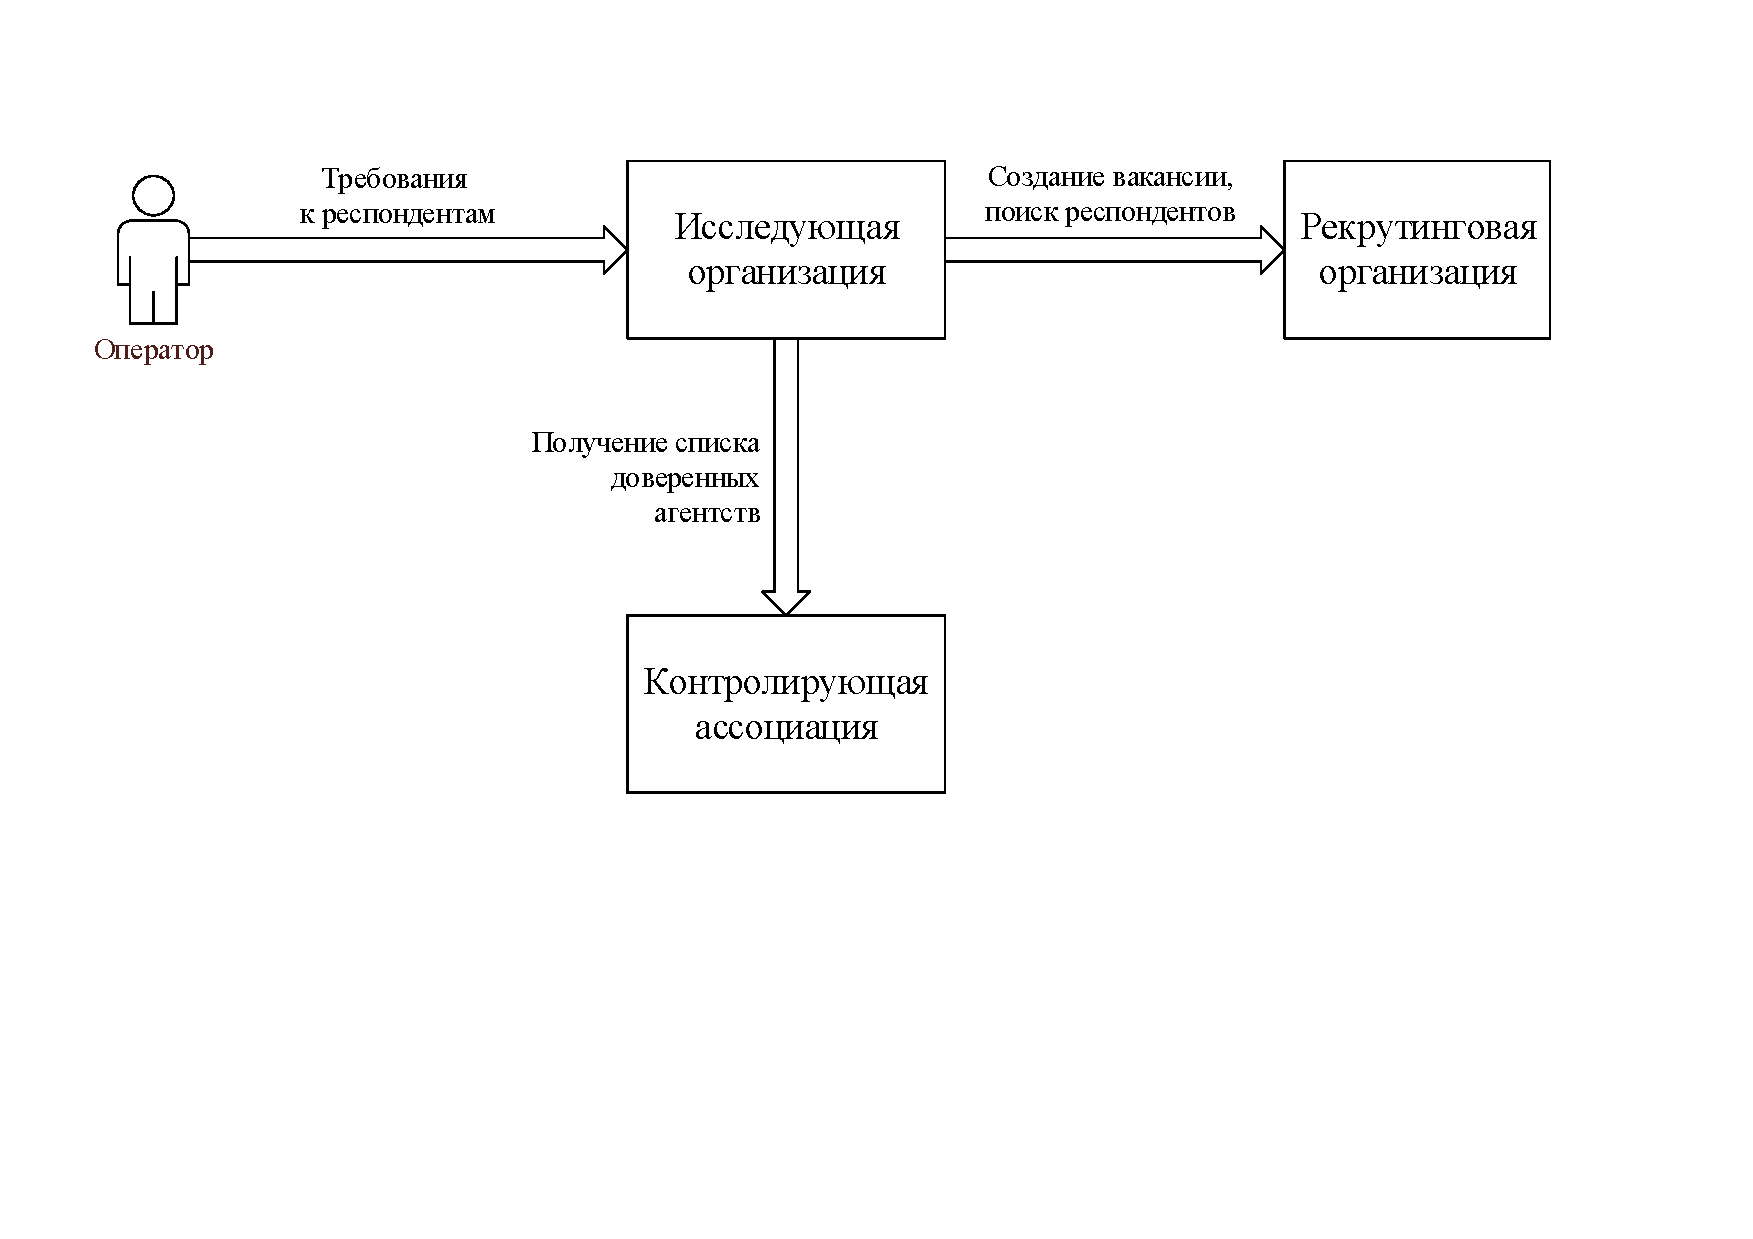
\includegraphics[width=\textwidth]{include/sc-obl.pdf}
  \caption{Схема предметной области}
  \label{fig:sc-obl}
\end{figure}

\section{Описание системы}
Распределенная система состоит из  исследующей организации, рекрутинговых агентств и ассоциаций, контролирующих качество работы последних. В рамках данной работы будут реализованы все эти участники.

На рисунке ~\ref{fig:idef0} изображен процесс функционирования РСОИ. Используются следующие обозначения:
\begin{enumerate}
\item система A — система исследующей организации;
\item система B — система рекрутингового агентства; 
\item система C — система контролирующей ассоциации;
\end{enumerate}

\begin{figure}[ht]
  \centering
  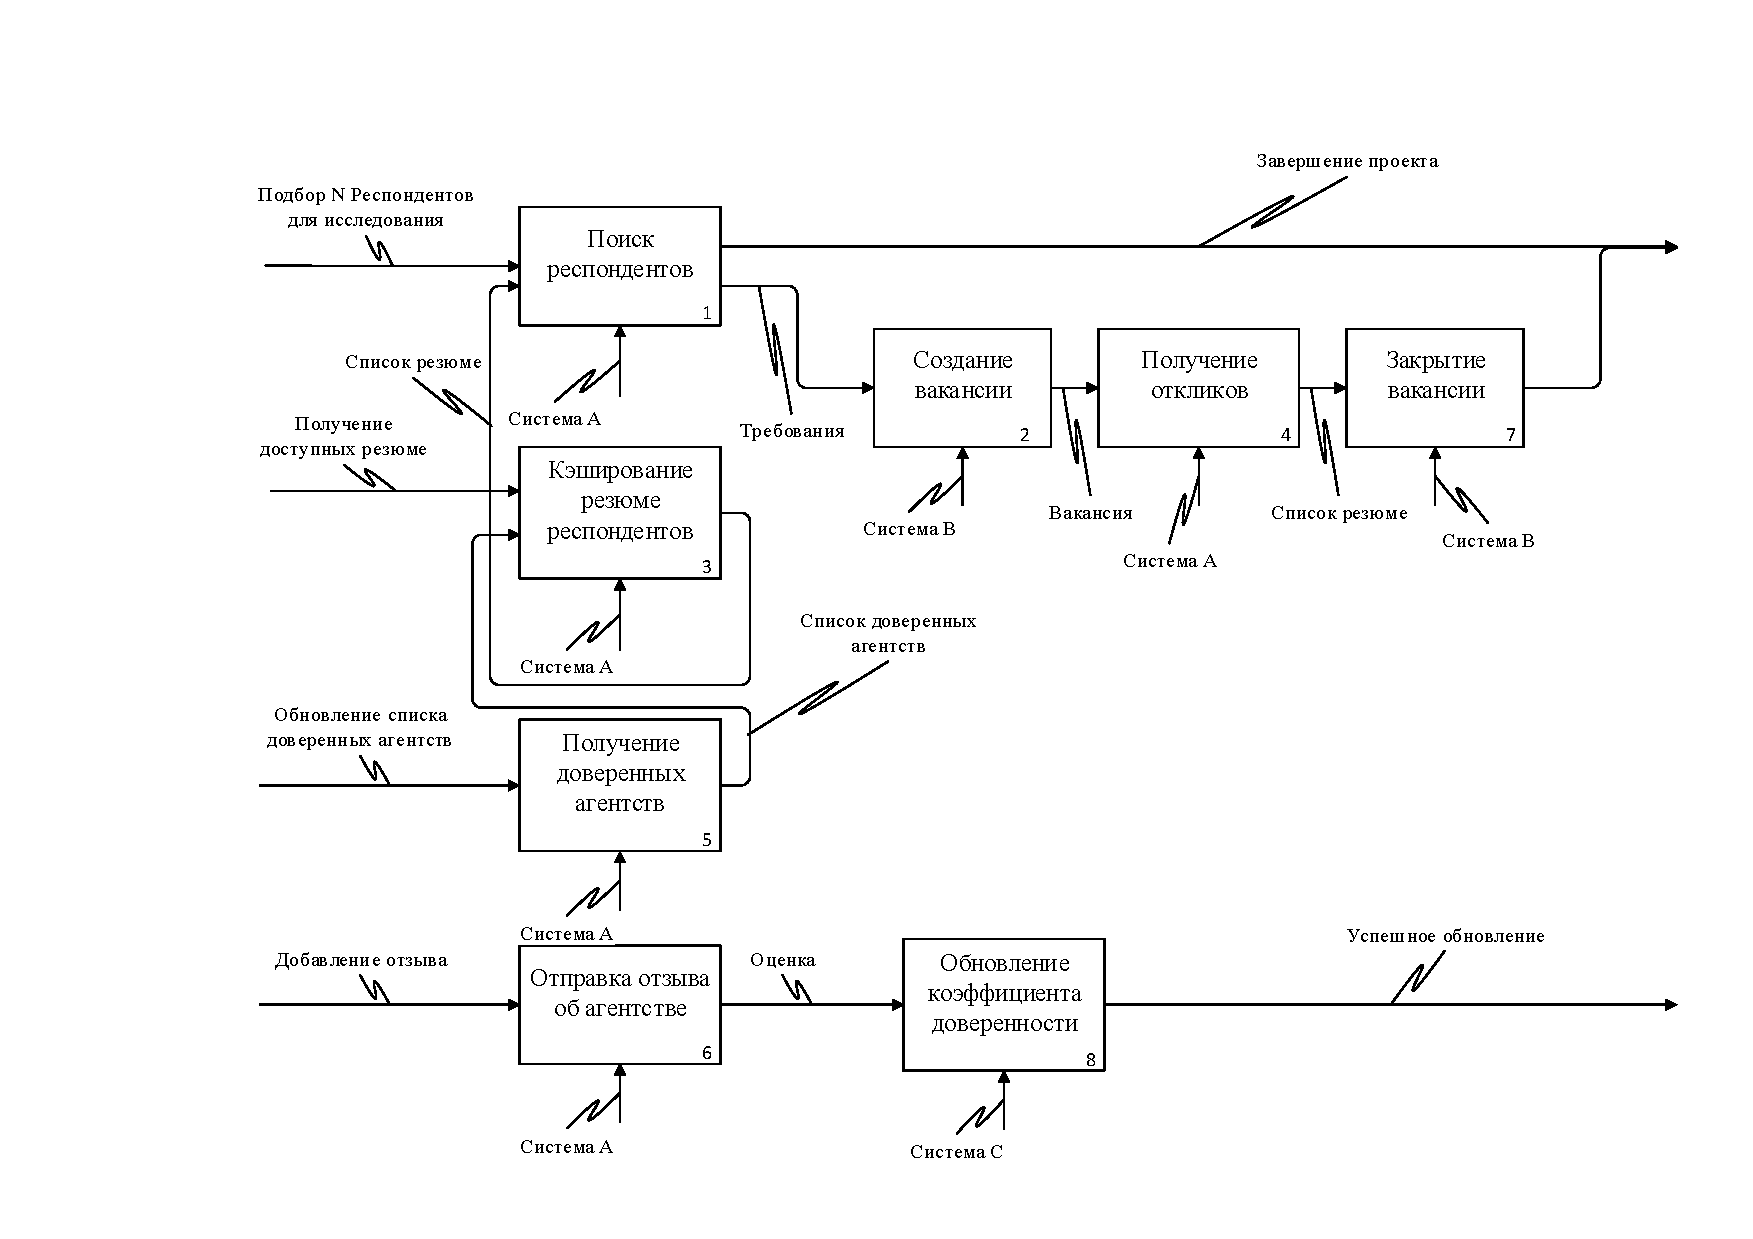
\includegraphics[width=\textwidth]{include/idef0.pdf}
  \caption{Диаграмма функционирования системы}
  \label{fig:idef0}
\end{figure}

Рассмотрим функционирование каждого участника РСОИ.
\begin{enumerate}[1.]
\item Система исследующей организации ~--- предоставляет оператору веб-интерфейс для управления исследованиями, модификации внутренней базы респондентов и создания вакансий для рекрутинговых агентств. Система взаимодействует с рекрутинговыми агентствами и ассоциациями контроля качества услуг. При этом должен быть предусмотрен контроль занятости респондентов, не позволяющий участвовать им одновременно в разных исследованиях. Позволяет оператору изменять и удалять проекты.
\item Система рекрутингового агентства ~--- предоставляет исследующей организации список подходящих респондентов. Множество подходящих людей выбирается автоматически на основе пришедших критерией, участие в конкретном исследовании подтверждается лично респондентом. Система содержит веб-интерфейс пользователя и администратора.
\item Система контролирующей ассоциации ~--- предоставляет исследующей организации данные о надежности рекрутинговых агентств. Собирает данные о работе рекрутинговых агентств (и других организаций, не рассматриваемых в данной работе).
\end{enumerate}

Основной сценарий взаимодействия пользователя с системой представляет собой последовательность следующих действий:
\begin{enumerate}
\itemоператор создает новый проект и определяет требования к респондентам;
\itemсистема выдает набор респондентов из внутренней базы, если этого недостаточно ~--- запрашивается список подходящих людей из рекрутинговых агентств, имеющих высокую оценку качества услуг, там же создается соответствующая вакансия;
\itemсистема рекрутингового агентства подбирает подходящих респондентов и рассылает им уведомления. При подтверждении от респондента его данные начинают выдаваться системе, создавшей вакансию;
\itemоператор договаривается с респондентами, изменяя их статус во внутренней базе;
\itemпо окончании проекта закрываются все вакансии, в рекрутинговые агентства отсылаются данные о реальных участниках исследования;
\itemтакже по окончании проекта оператор может отослать отзыв о качестве услуг рекрутеров;
\itemсистема исследующей организации при получении данных об ухудшении качества работы закрывает все вакансии и прекращает создание новых; при получении данных о новой рекрутинговой компании открывает вакансии там со следующего проекта
\end{enumerate}

В случае закрытия проекта (например, в случае разрыва контракта с клиентом) закрываются все открытые вакансии в рекрутинговых агентствах, а уже отобранным респондентам отсылается письмо с сообщением об этом прискорбном факте.

\section{Требования к системе}
На основе анализа предметной области необходимо сформулировать требования как к всей системе, так и к ее подсистемам.

\subsection{Требования к системе в целом}
\begin{enumerate}
\item Система должна поддерживать добавление новых узлов.
\item Система не должна выходить из строя при выходе из строя одной из подсистем.
\item Обмен информации в системе должен производиться исходя из предположения, что каналы связи небезопасны и ненадежны.
\item Система должна предусматривать восстановление в случае сбоя.
\end{enumerate}

\subsection{Требования к системе экскурсионного бюро}

\textbf{Функциональные требования}
\begin{enumerate}
\item Система должна предоставлять оператору веб-интерфейс.
\item Система должна осуществлять  аутентификацию пользователей по электронной почте/паролю, добавление новых операторов доступно только администратору.
\item Оператор должен видеть список открытых текущих проектов, информацию об отобранных/требуемых респондентах.
\item Система должна предоставлять оператору возможность изменения внутренней базы респондентов.
\item Система должна предоставлять возможность отправить отзыв о рекрутинговой компании в контролирующую ассоциацию.
\end{enumerate}

\textbf{Входные данные}
\begin{enumerate}
\item Требования к респондентам:
\begin{enumerate}
\item пол;
\item возраст;
\item профессия;
\item доход;
\item прочие особенности (ключевые слова).
\end{enumerate}
\item Количество респондентов, требуемых для исследования:
\end{enumerate}

\textbf{Выходные данные}
\begin{enumerate}
\item список респондентов, отобранных по внутренней базе;
\item список респондентов, присланных из рекрутинговых агентств;
\item коэффициента доверия рекрутинговому агентству, подобравшему респондента
\end{enumerate}

\subsection{Требования к системе рекрутингового агентства}

\textbf{Функциональные требования}
\begin{enumerate}
\item Система должна подбирать респондентов по присланным критериям автоматически.
\item Пользователи могут принимать предложения от исследующей организации или отказываться.
\end{enumerate}

\textbf{Входные данные}
\begin{enumerate}
\item описание исследования;
\item требования к респонденту;
\end{enumerate}

\textbf{Выходные данные}
\begin{enumerate}
\item список подходящих респондентов;
\item список согласившихся респондентов.
\end{enumerate}

\subsection{Требования к системе контролирующей ассоциации}

\textbf{Функциональные требования}
\begin{enumerate}
\item Система должна предоставлять список всех контролируемых организаций с коэффициентами доверия.
\item Система должна собирать отзывы о компаниях от других систем или пользователей.
\end{enumerate}

\textbf{Входные данные}
\begin{enumerate}
\item название контролируемой организации;
\item отзыв.
\end{enumerate}

\textbf{Выходные данные}
\begin{enumerate}
\item список контролируемых организаций с оценками надежности;
\end{enumerate}

\section{Сценарии использования системы}
В качестве пользователей системы выступают операторы исследующей системы, которые формируют требования к респондентам. В дальнейшем будем называть их просто "оператор". 

Рассмотрим возможные сценарии:

\textbf{"Вход в систему"}

Краткое описание: оператор входит в систему под своим Google аккаунтом.

\textbf{Сценарий:}\\
Основной поток:
\begin{enumerate}
\item оператор переходит на страницу авторизации исследующей системы. Формируется заявка на OAuth.
\item далее он переходит на сайт Google и выбирает почту, с помощью которой он хочет войти;
\item Google  возвращает данные авторизации системе;
\item если данные от Google получены, соответствующий email содержится в базе, а номер заявки на авторизацию существует в системе — оператор переходит на страницу управления проектами.
\end{enumerate}
Альтернативный поток:
\begin{enumerate}
\item оператор выбирает почту на сайте Google, с помощью которой он хочет войти;
\item Google возвращает данные об авторизации системе;
\item если код авторизации отсутствует, либо соответствующий email или номер заявки на авторизацию отсутствует в базе — выводится сообщение об ошибке, оператор остается на странице входа.
\end{enumerate}

\textbf{"Создание проекта"}

Краткое описание: оператор создает новый проект и заполняет требования к респондентам.

\textbf{Сценарий:}\\
Основной поток:
\begin{enumerate}
\item оператор входит в систему;
\item оператор вводит название проекта, требования к респондентам и их количество;
\item система осуществляет поиск по внутренней базе респондентов;
\item в случае, если подходящих респондентов во внутренней базе мало, система создает заявки в доверенных рекрутинговых агентствах;
\item кроме того, осуществляется поиск по кэшированным данным респондентов из рекрутинговых агентств;
\item система выводит результаты поиска и ассоциированные вакансии на экран.
\end{enumerate} 

\textbf{"Отклик на вакансию"}

Краткое описание: респондент из рекрутингового агентства оставил отклик на вакансию.

\textbf{Сценарий:}\\
Основной поток:
\begin{enumerate}
\item система осуществляет опрос рекрутинговых агентств и получает список новых откликов;
\item новые отклики добавляются в список возможных респондентов проекта;
\item оператор обрабатывает новые данные — обзванивает подобранных респондентов или осуществляет рассылку;
\end{enumerate} 

\textbf{"Неуспешное завершение проекта"}

Краткое описание: по неизвестным причинам оператор завершает проект как неуспешный.

\textbf{Сценарий:}\\
Основной поток:
\begin{enumerate}
\item оператор завершает проект как неуспешный;
\item система закрывает все ассоциированные с проектом вакансии;
\item система отсылает письмо всем отобранным респондентам о том, что проект более не существует;
\item система удаляет данные о подходящих и отобранных респондентах для проекта;
\item по желанию оператора оставляется отзыв об использованных рекрутинговых компаниях.
\end{enumerate}

\textbf{"Успешное завершение проекта"}

Краткое описание: исследование было проведено успешно, оператор закрывает проект.

\textbf{Сценарий:}\\
Основной поток:
\begin{enumerate}
\item оператор завершает проект как успешный;
\item система закрывает все ассоциированные с проектом вакансии;
\item система удаляет данные о подходящих и отобранных респондентах для проекта;
\item по желанию оператор может оставить отзыв об использованных рекрутинговых компаниях.
\end{enumerate}

\textbf{"Изменение списка доверенных рекрутинговых агентств"}

Краткое описание: при обновлении данных из контролирующей ассоциации появилось новое доверенное агентство с заданным рейтингом доверия либо уже известное агентство получило рейтинг доверия ние допустимого.

\textbf{Сценарий:}\\
Основной поток:
\begin{enumerate}
\item система получает список рекрутинговых агентств от контролирующей ассоциации;
\item если используемое рекрутинговое агентство получило рейтинг ниже допустимого - все открытые вакансии и кэшированная база респондентов удаляется, этот участник больше не используется в РСОИ;
\item если появилось новое рекрутинговое агентсво с достаточным рейтингов - для текущих проектов в нем создаются вакансии, обновляется кэшированная база респондентов. Также новый участник используется в РСОИ для последующих проектов.
\end{enumerate}

%%% Local Variables:
%%% mode: latex
%%% TeX-master: "rpz"
%%% End:

\chapter{Конструкторский раздел}
\label{cha:design}

В данном разделе описывается процесс проектирования субъектов разрабатываемой распределенной системы: системы исследующей организации, системы рекрутингового агентства и системы контролирующей ассоциации, а также их взаимодействия.

\section{Архитектура разрабатываемой распределенной системы}

Разрабатываемая распределенная система состоит из субъектов трех видов: системы исследующей организации, системы рекрутингового агентства и системы контролирующей ассоциации. Архитектура системы представлена на рисунке~\ref{fig:arch}.

\begin{figure}[ht]
  \centering
  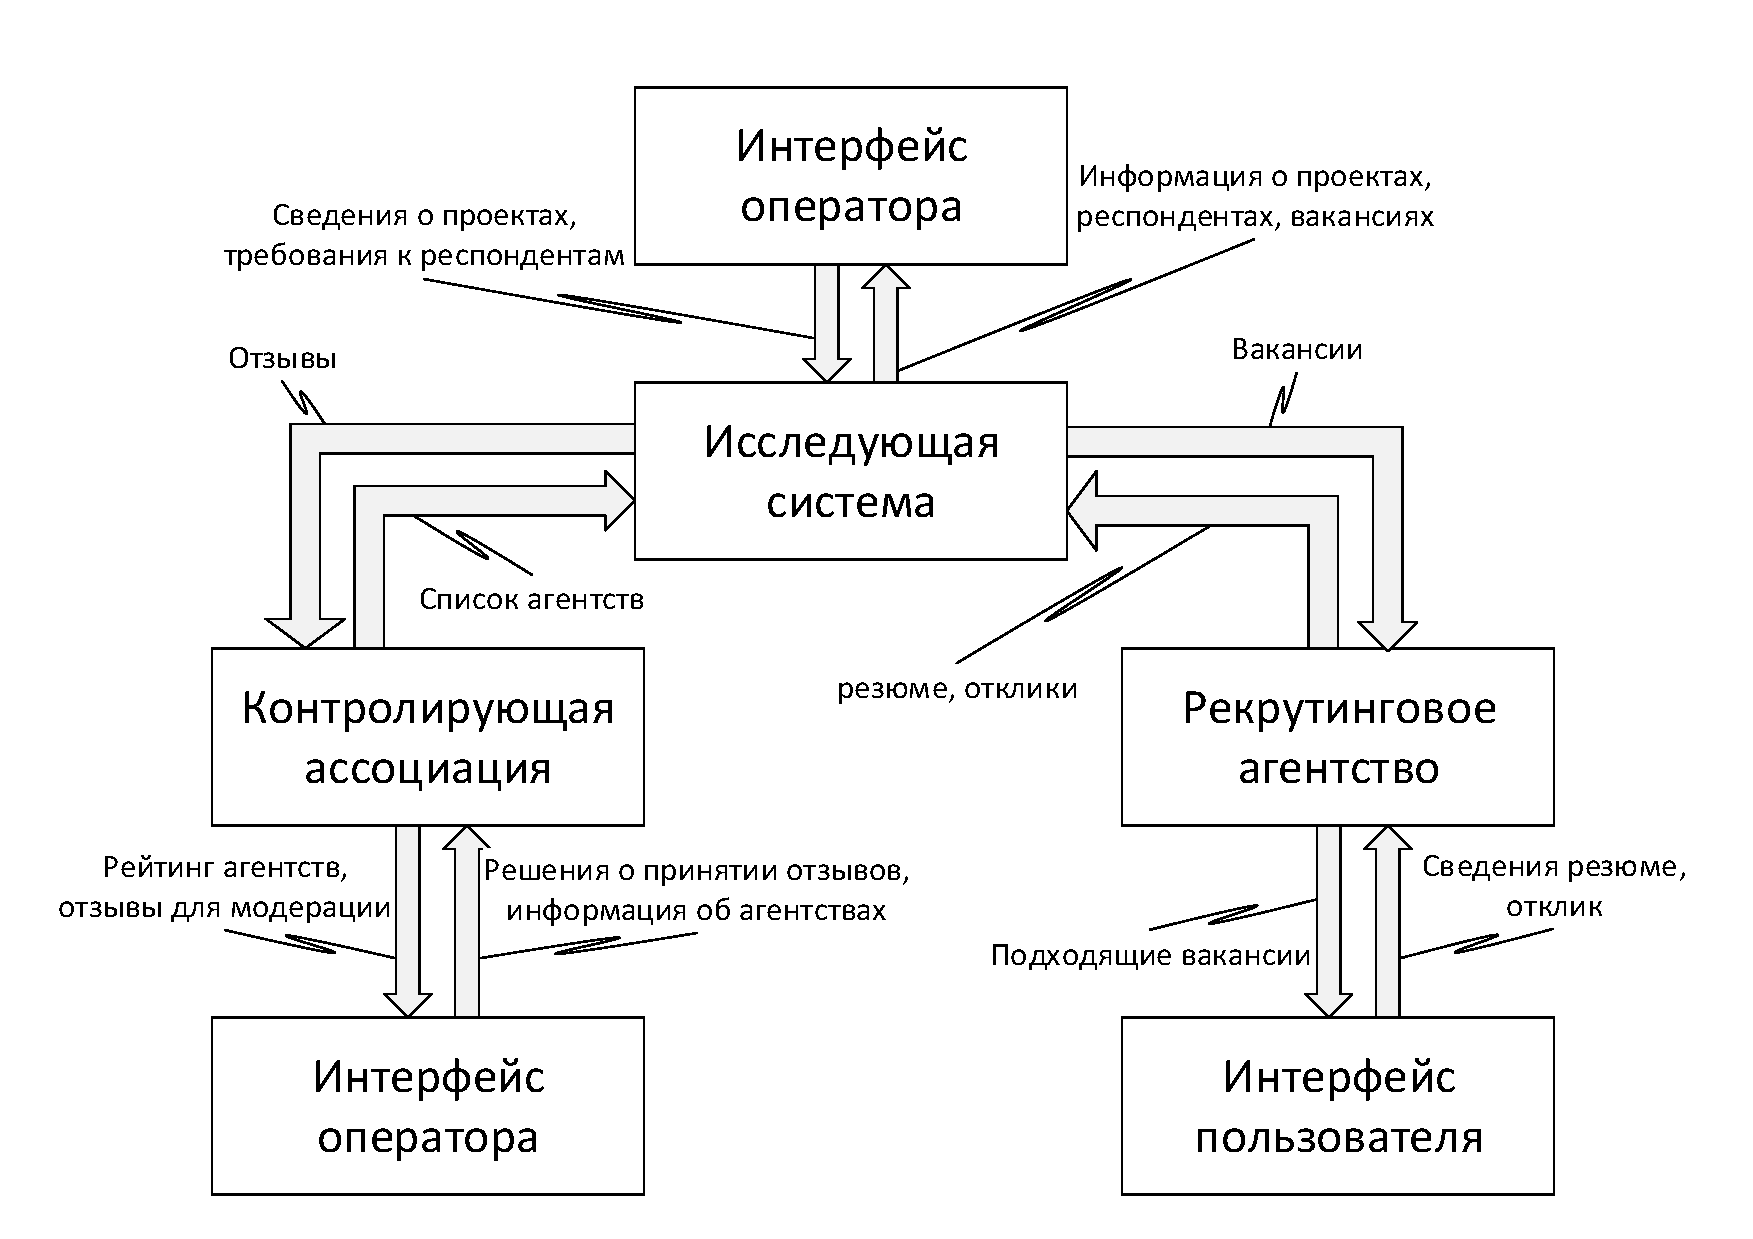
\includegraphics[width=\textwidth]{include/arch.pdf}
\caption{Архитектура системы}
\label{fig:arch}
\end{figure}

\textbf{Система исследующей организации} осуществляет создание проектов, поиск подходящих респондентов, размещение заявок и отправку отзывов о рекрутинговых агентствах. Система предоставляет операторы Web-интерфейс для создания проекта и отбора респондентов, а также для отправки отзывов. 

\textbf{Система рекрутингового агентства} предоставляет системе исследующей организации резюме респондентов, по запросу создает или закрывает вакансию, выдает список откликов. Предоставляет интерфейс пользователя для регистрации, редактирования резюме и отклика на вакансию. 

\textbf{Система контролирующей ассоциации} предоставляет исследующей организации информацию о доверенных рекрутинговых агентствах, принимает отзывы о них и обновляет рейтинг. Предоставляет интерфейс администратора для изменения информации об агентствах и модерации отзывов.

\section{Протокол взаимодействия систем} 
Субъекты РСОИ должны взаимодействовать по формализованному протоколу взаимодействия. В этом параграфе описывается последовательность и формат передаваемых сообщений. 

\subsection{Последовательность передаваемых сообщений}
Для реализации взаимодействия субъектов распределенной системы друг с другом используется как синхронный так и асинхронный подход. Рассмотрим варианты взаимодействия, проиллюстрированные на диаграммах последовательностей.

\paragraph{Случай 1. Поиск респондентов для проекта}

При поиске респондентов для проекта система исследующей организации осуществляет периодическое кеширование списка доверенных рекрутинговых агентств и резюме в них. Затем по запросу пользователя создается вакансия во всех доверенных рекрутинговых агентствах, до ее закрытия периодически проверяются отклики. После завершения проекта отправляется сообщение о закрытии вакансии.
Диаграмма последовательности для поиска респондентов показана на рисунке ~\ref{fig:sequence1}.
\begin{figure}[ht]
  \centering
  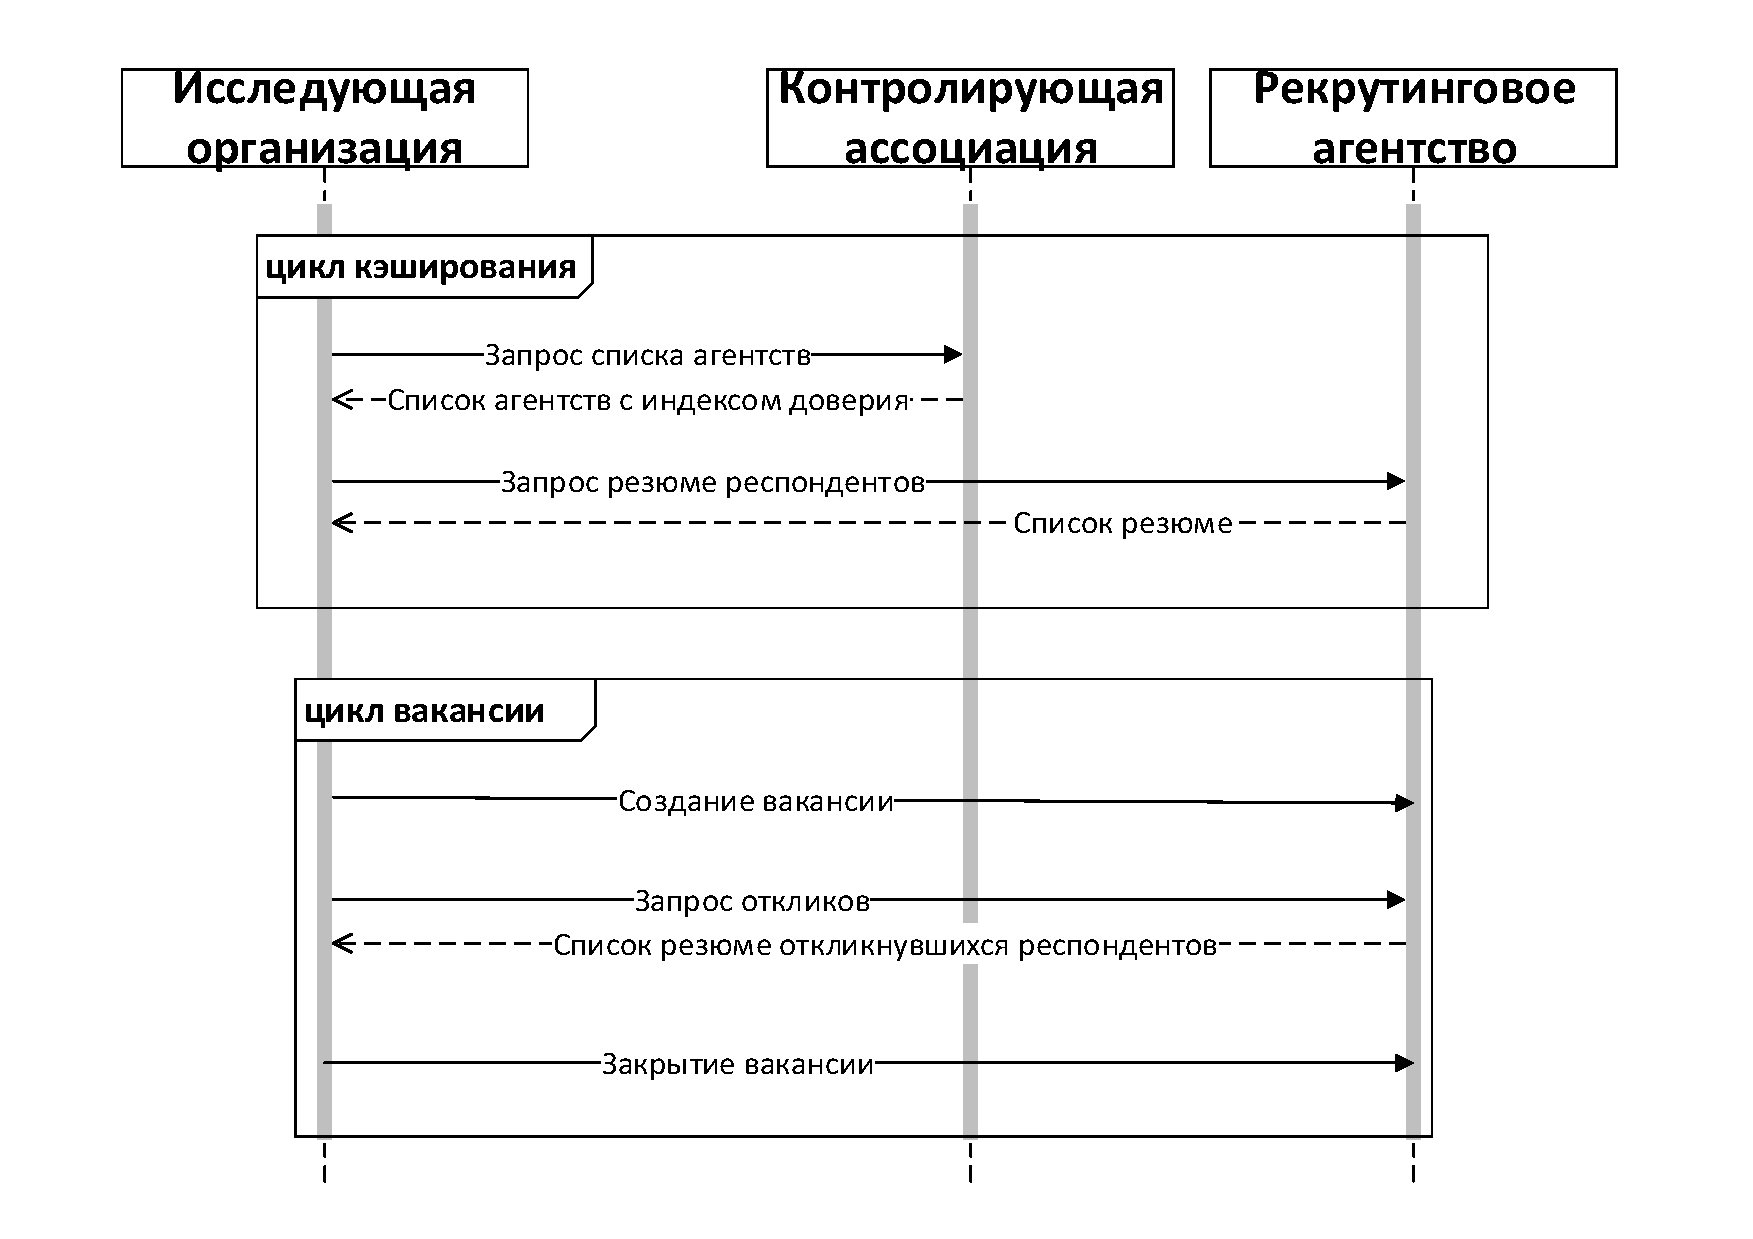
\includegraphics[width=\textwidth]{include/sequence1.pdf}
\caption{Диаграмма последовательности для подбора респондентов}
\label{fig:sequence1}
\end{figure}

\paragraph{Случай 2. Отправка отзыва и обновление рейтинга}

Периодически осуществляется кеширование списка рекрутинговых агентств. По запросу пользователя посылается асинхронный запрос с отзывом и оценкой конкретному агентству. После модерации отзыва в контролирующей ассоциации обновляется рейтинг доверия указанной системе, который будет обновлен при следующем кешировании.  
Диаграмма последовательности для отправки отзыва показана на рисунке ~\ref{fig:sequence2}.

\begin{figure}[ht]
  \centering
  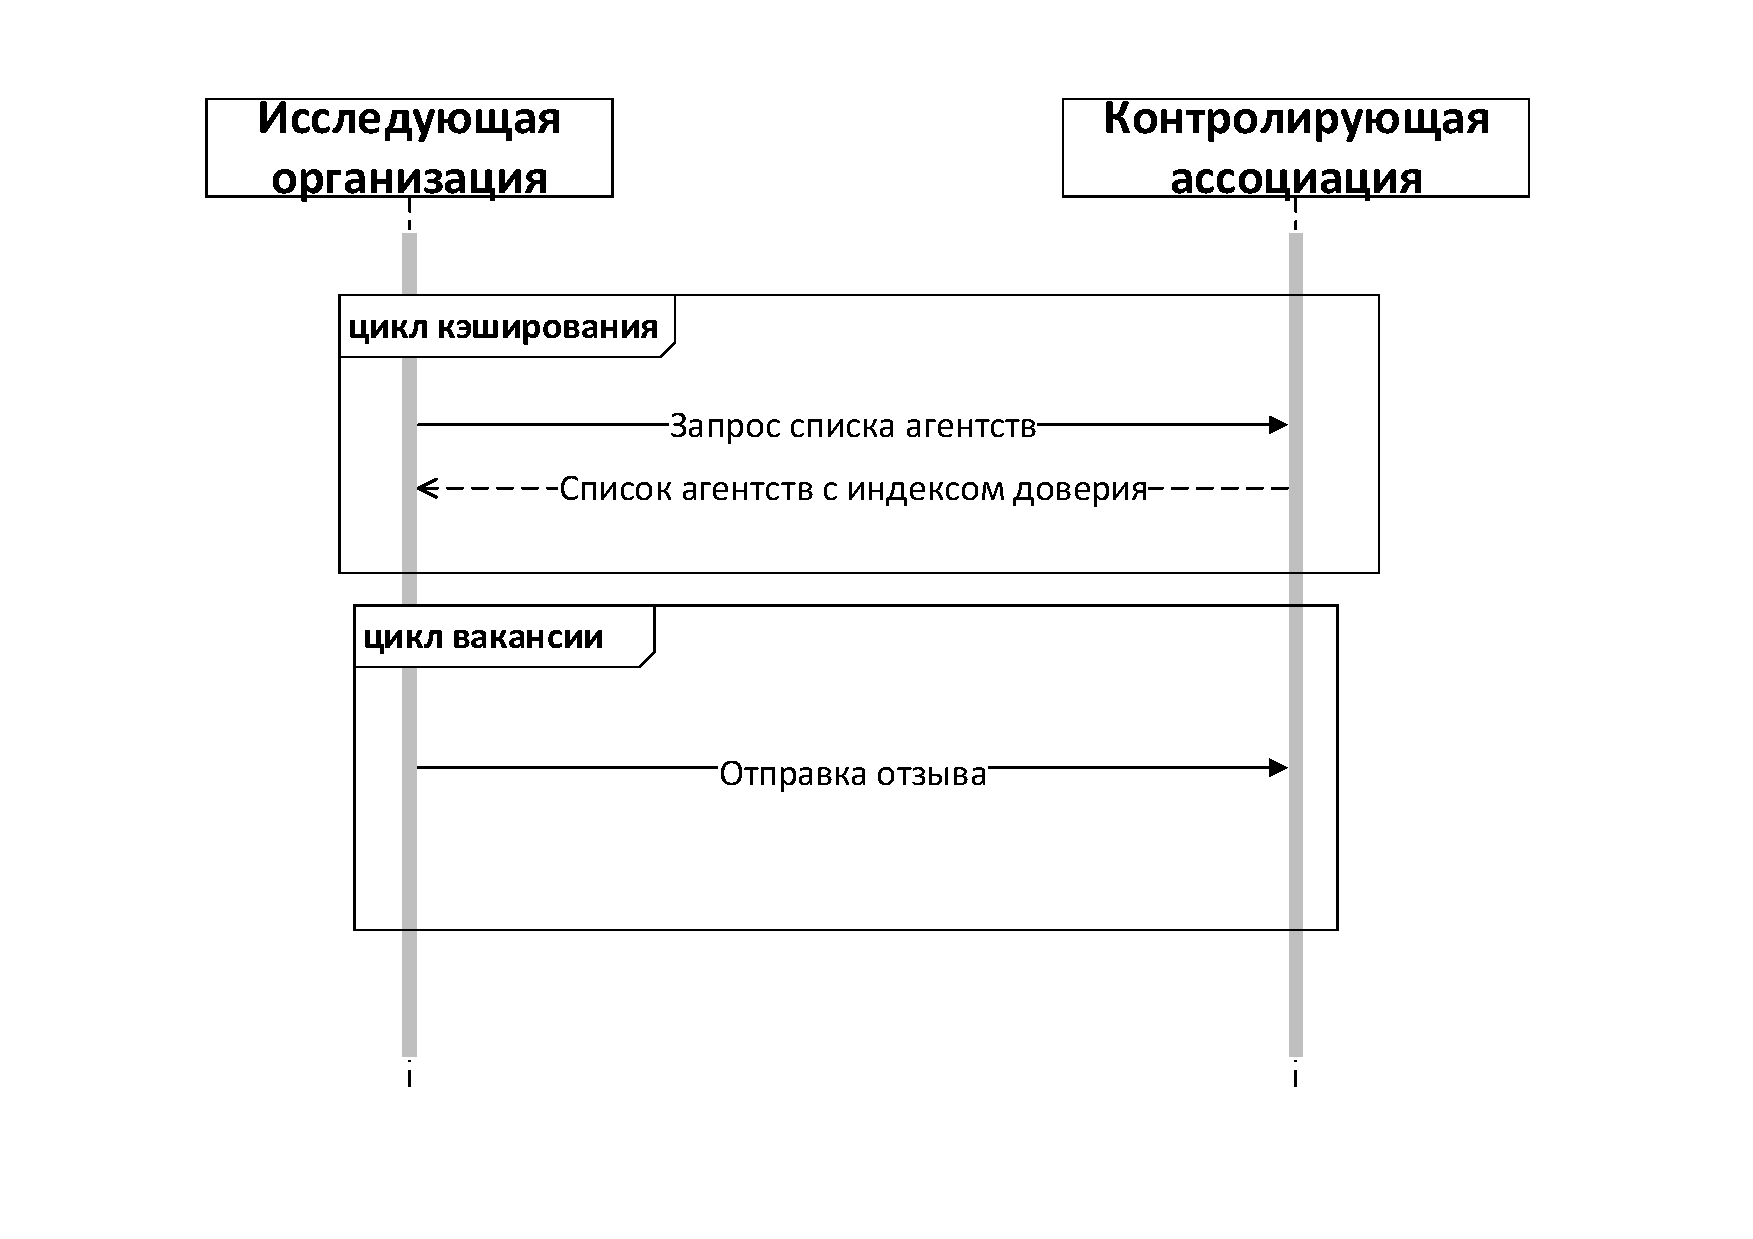
\includegraphics[width=\textwidth]{include/sequence2.pdf}
\caption{Диаграмма последовательности для отправки отзыва}
\label{fig:sequence2}
\end{figure}

\section{Система исследующей организации}
Данные системы исследующей организации содержат следующие сущности, связи которых представлены на рисунке ~\ref{fig:er-survey}, а описание атрибутов - на рисунке ~\ref{fig:er-survey-at}:

\begin{figure}[ht]
  \centering
  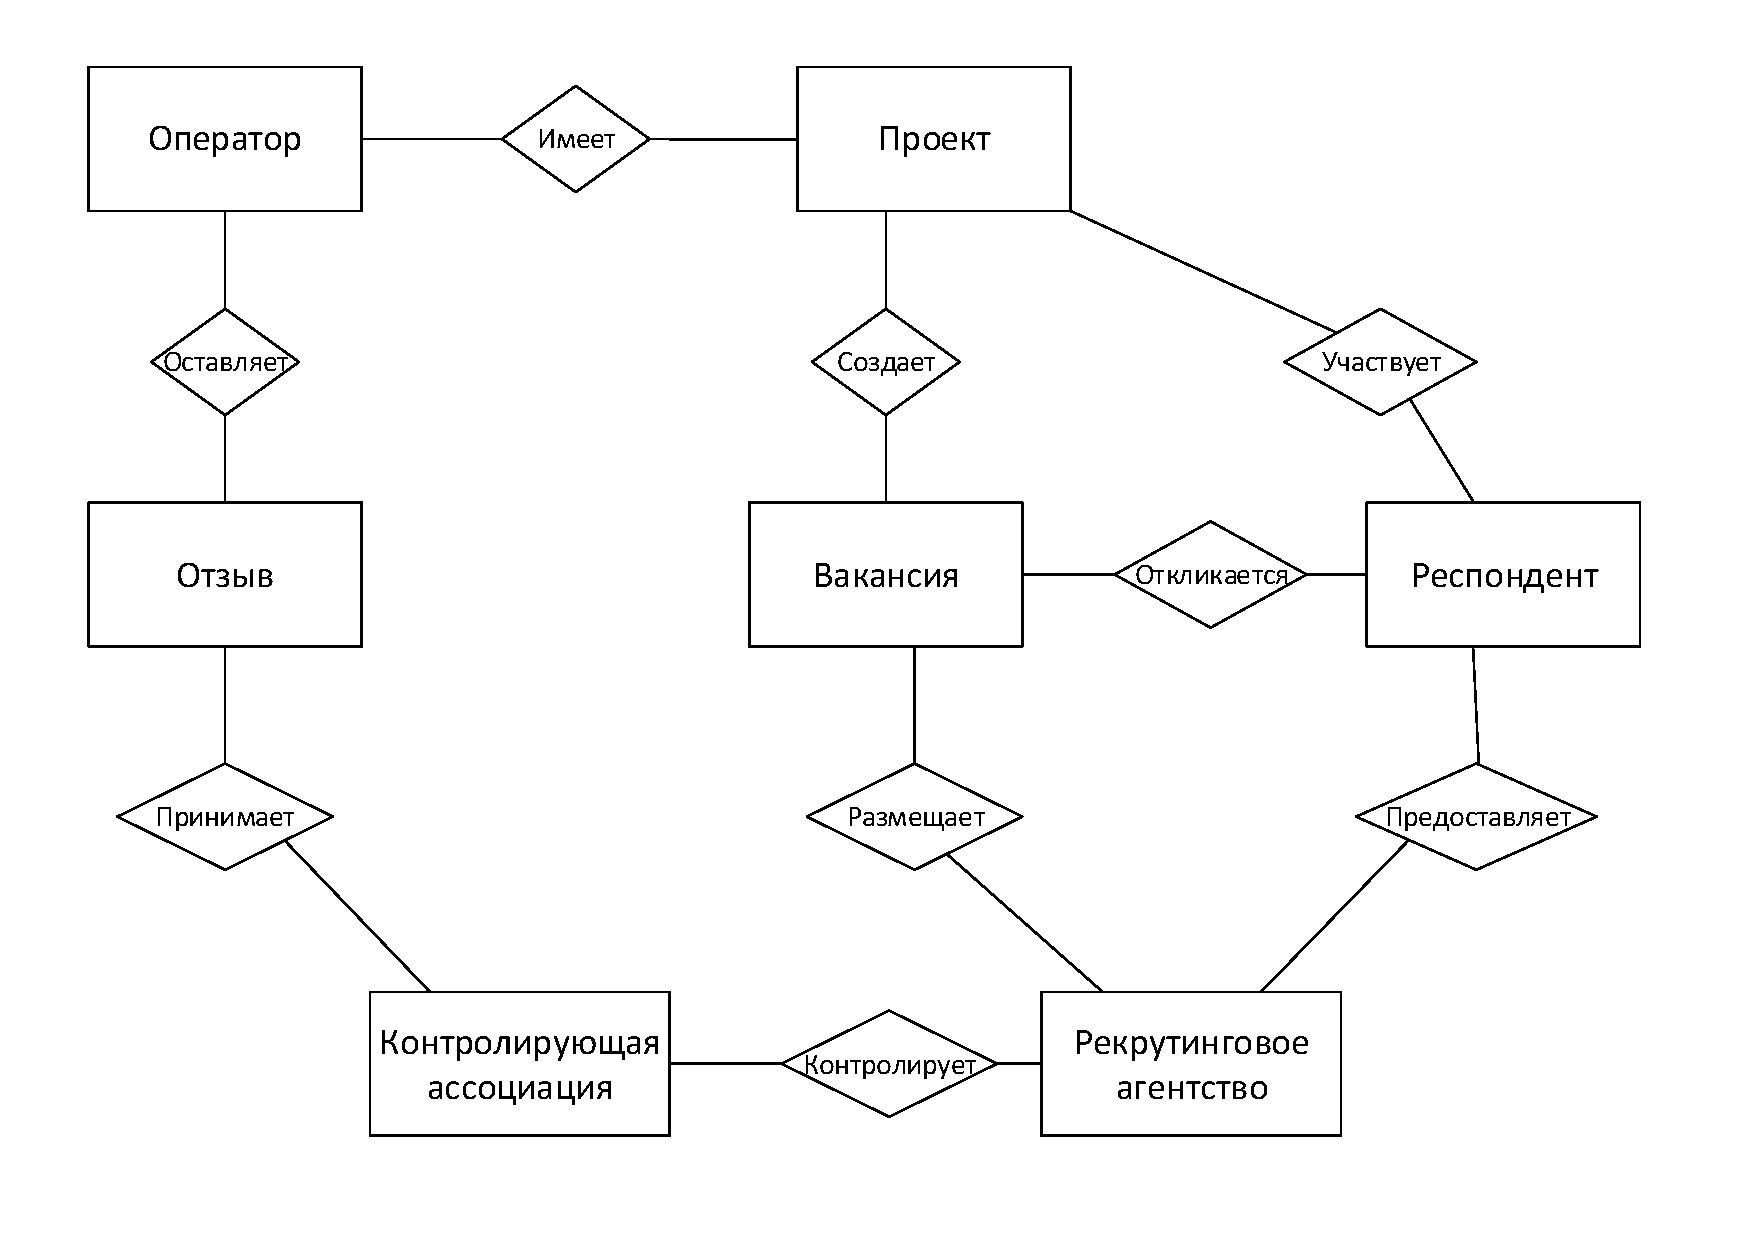
\includegraphics[width=\textwidth]{include/er-survey.pdf}
\caption{ER-диаграмма исследующей системы}
\label{fig:er-survey}
\end{figure}

\begin{figure}[ht]
  \centering
  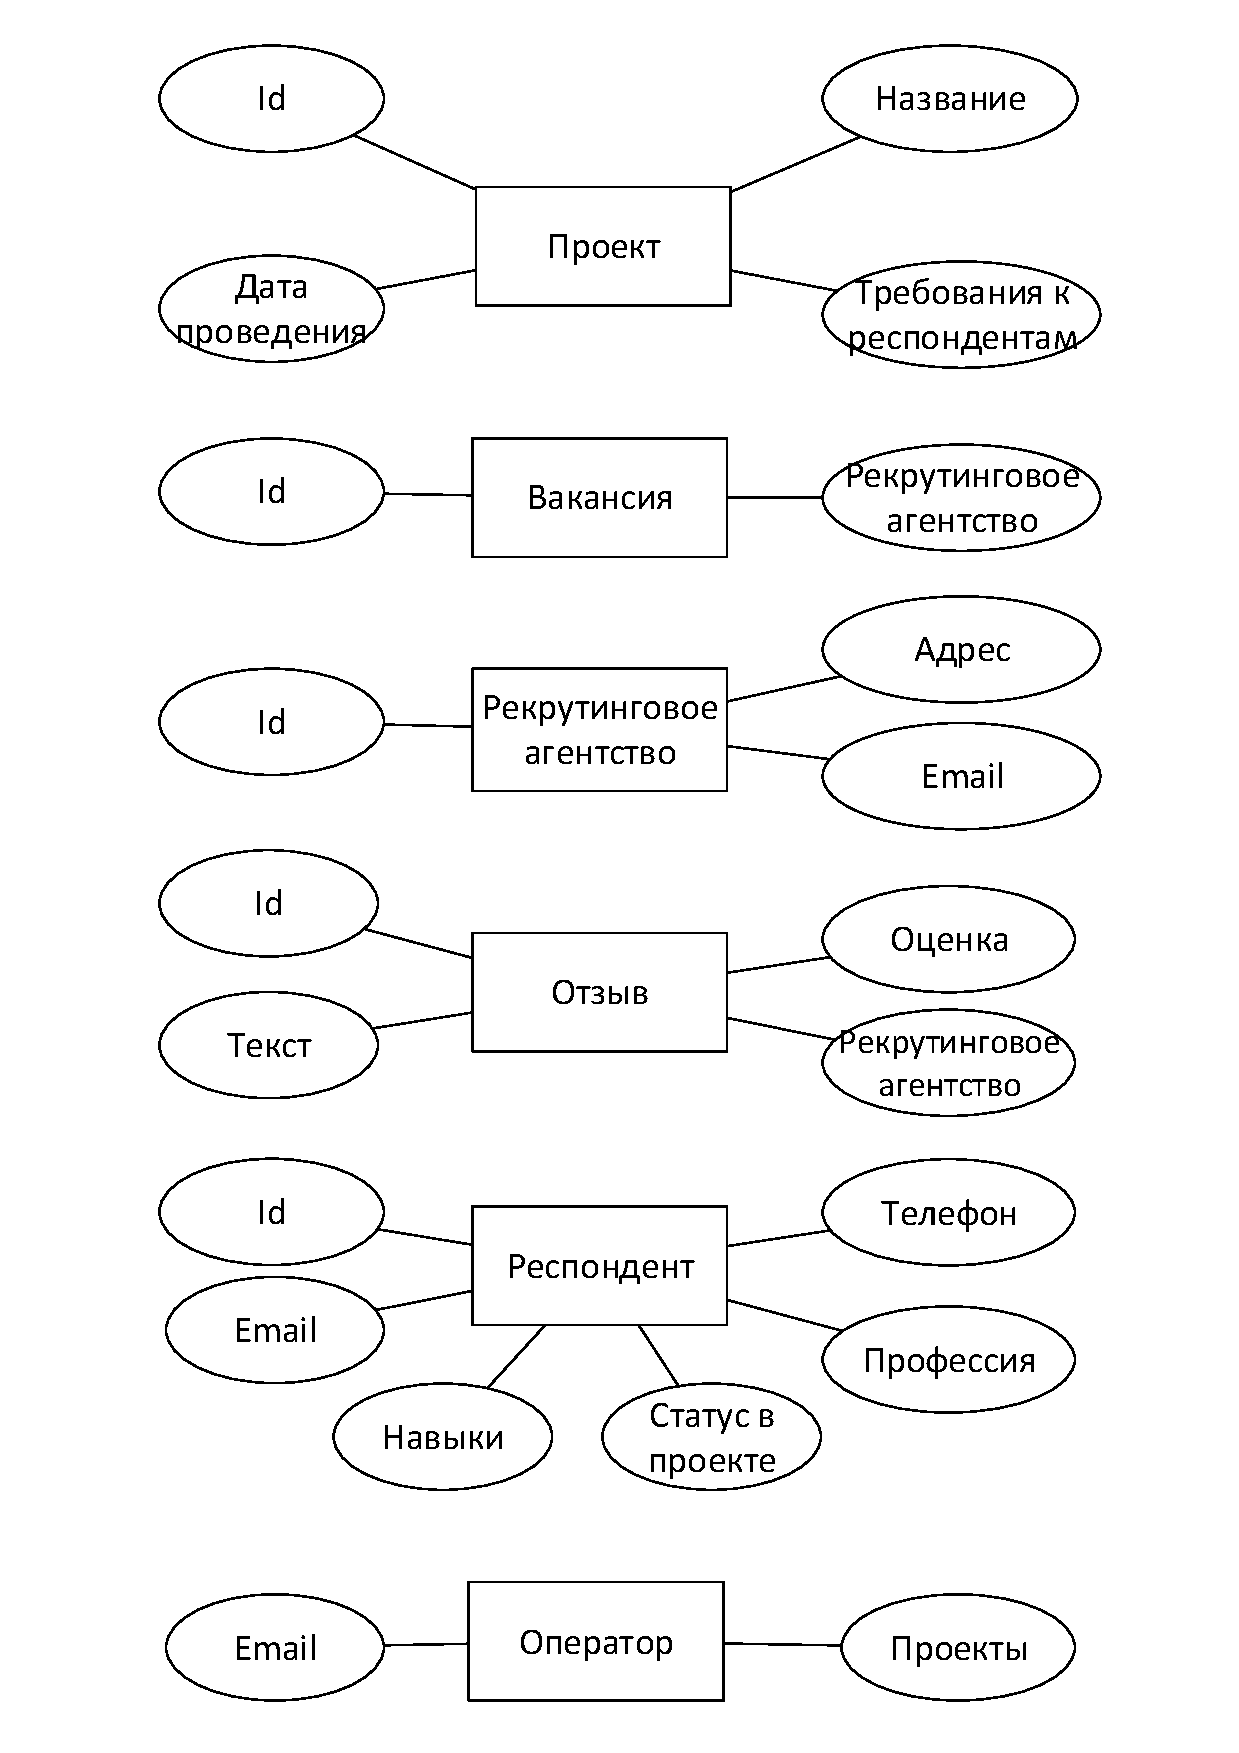
\includegraphics[width=\textwidth]{include/er-survey-at.pdf}
\caption{Атрибуты сущностей исследующей системы}
\label{fig:er-survey-at}
\end{figure}

\begin{enumerate}
\item оператор — имеет email и отображаемое имя, создает проекты и оставляет отзывы к рекрутинговым агентствам;
\item проект — имеет название, дату проведение и требования к респондентам, создает вакансии;
\item вакансия — создается в конкретном рекрутинговом агентстве и имеет ассоциированный проект;
\item рекрутинговое агентство — имеет адрес и email, предоставляется контролирующей ассоциацией;
\item отзыв — текст, оценка и id рекрутингового агентства в контролирующей ассоциации;
\item респондент — имеет имя, фамилию, email, телефон, профессию, навыки; может участвовать в проектах, откликаться на вакансии.
\end{enumerate}

\section{Система контролирующей ассоциации}
Данные системы контролирущей ассоциации содержат следующие сущности, связи которых представлены на рисунке ~\ref{fig:er-survey}, а описание атрибутов - на рисунке ~\ref{fig:er-survey-at}:

\begin{figure}[ht]
  \centering
  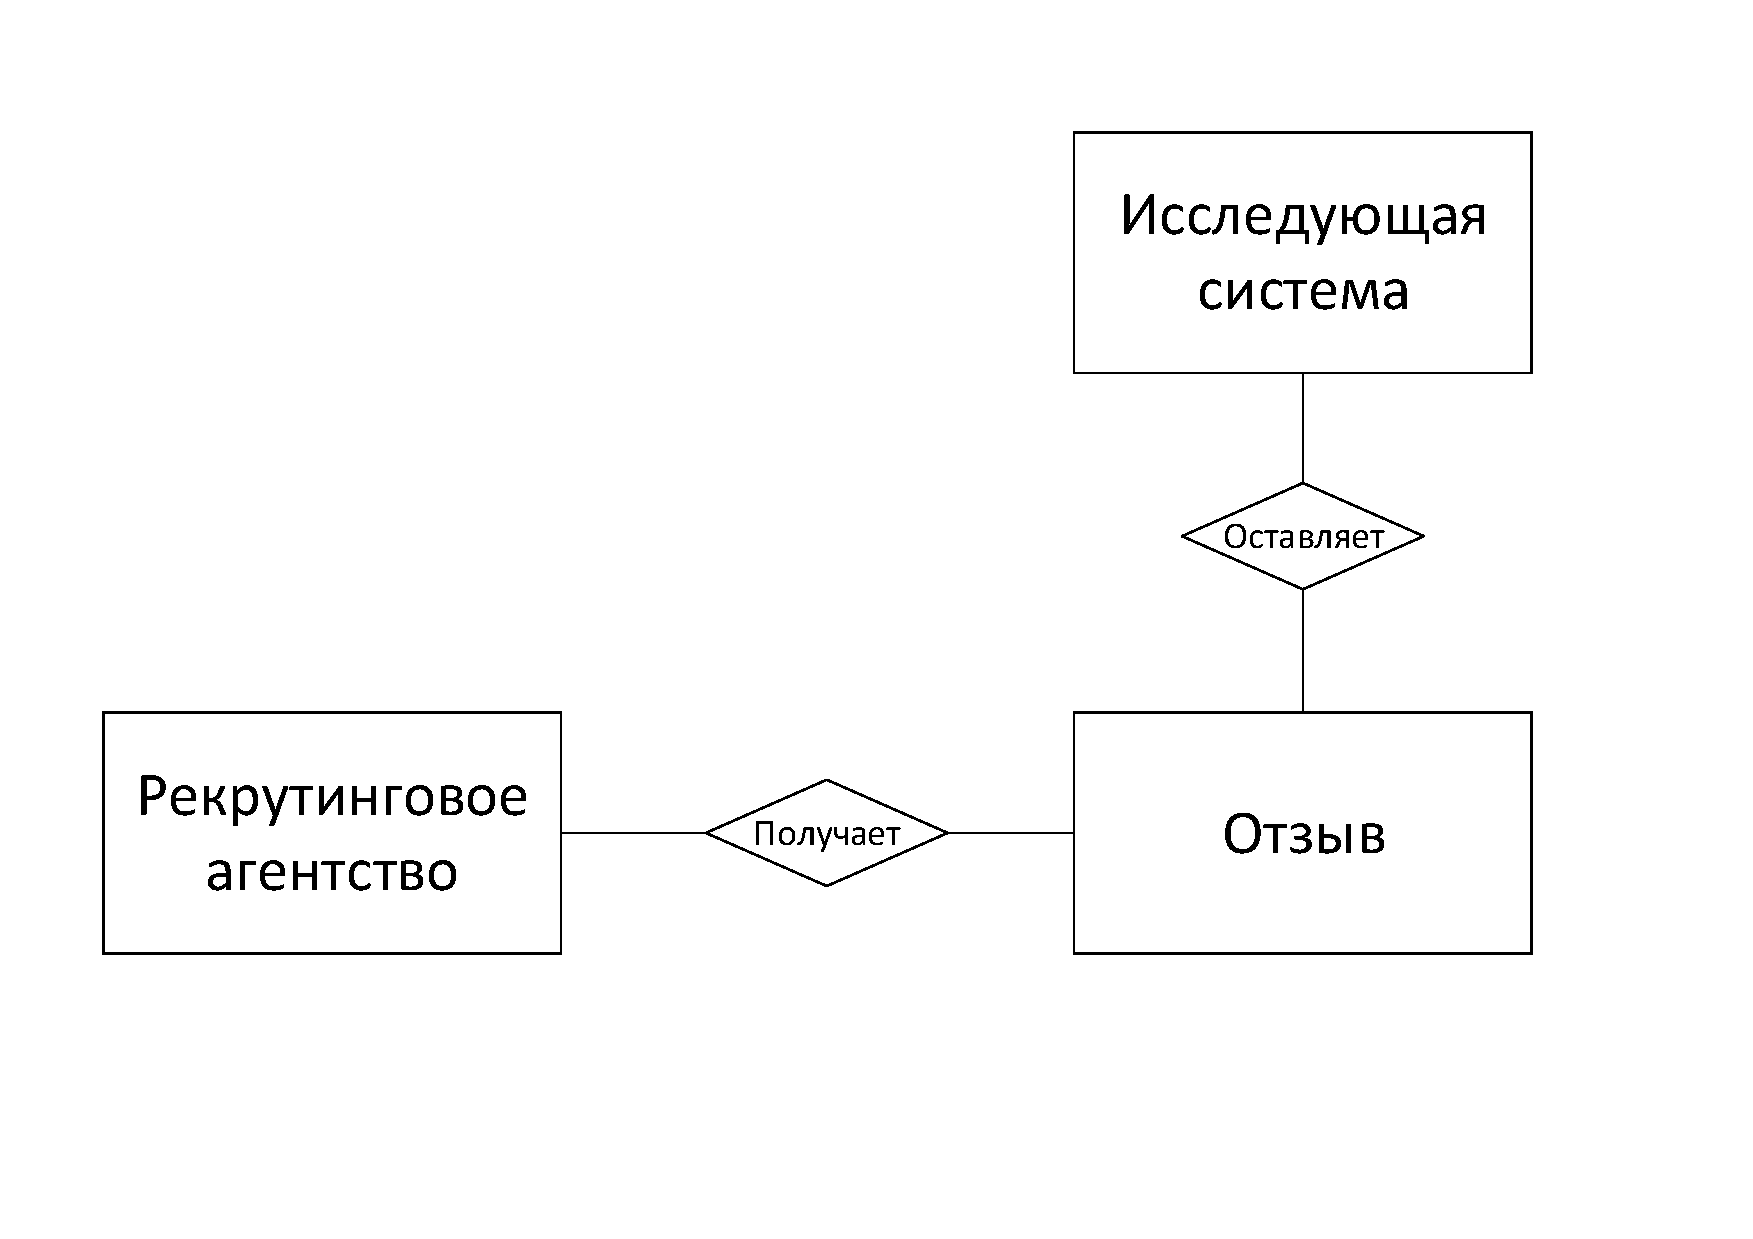
\includegraphics[width=\textwidth]{include/er-supervising.pdf}
\caption{ER-диаграмма контролирующей системы}
\label{fig:er-supervising}
\end{figure}

\begin{figure}[ht]
  \centering
  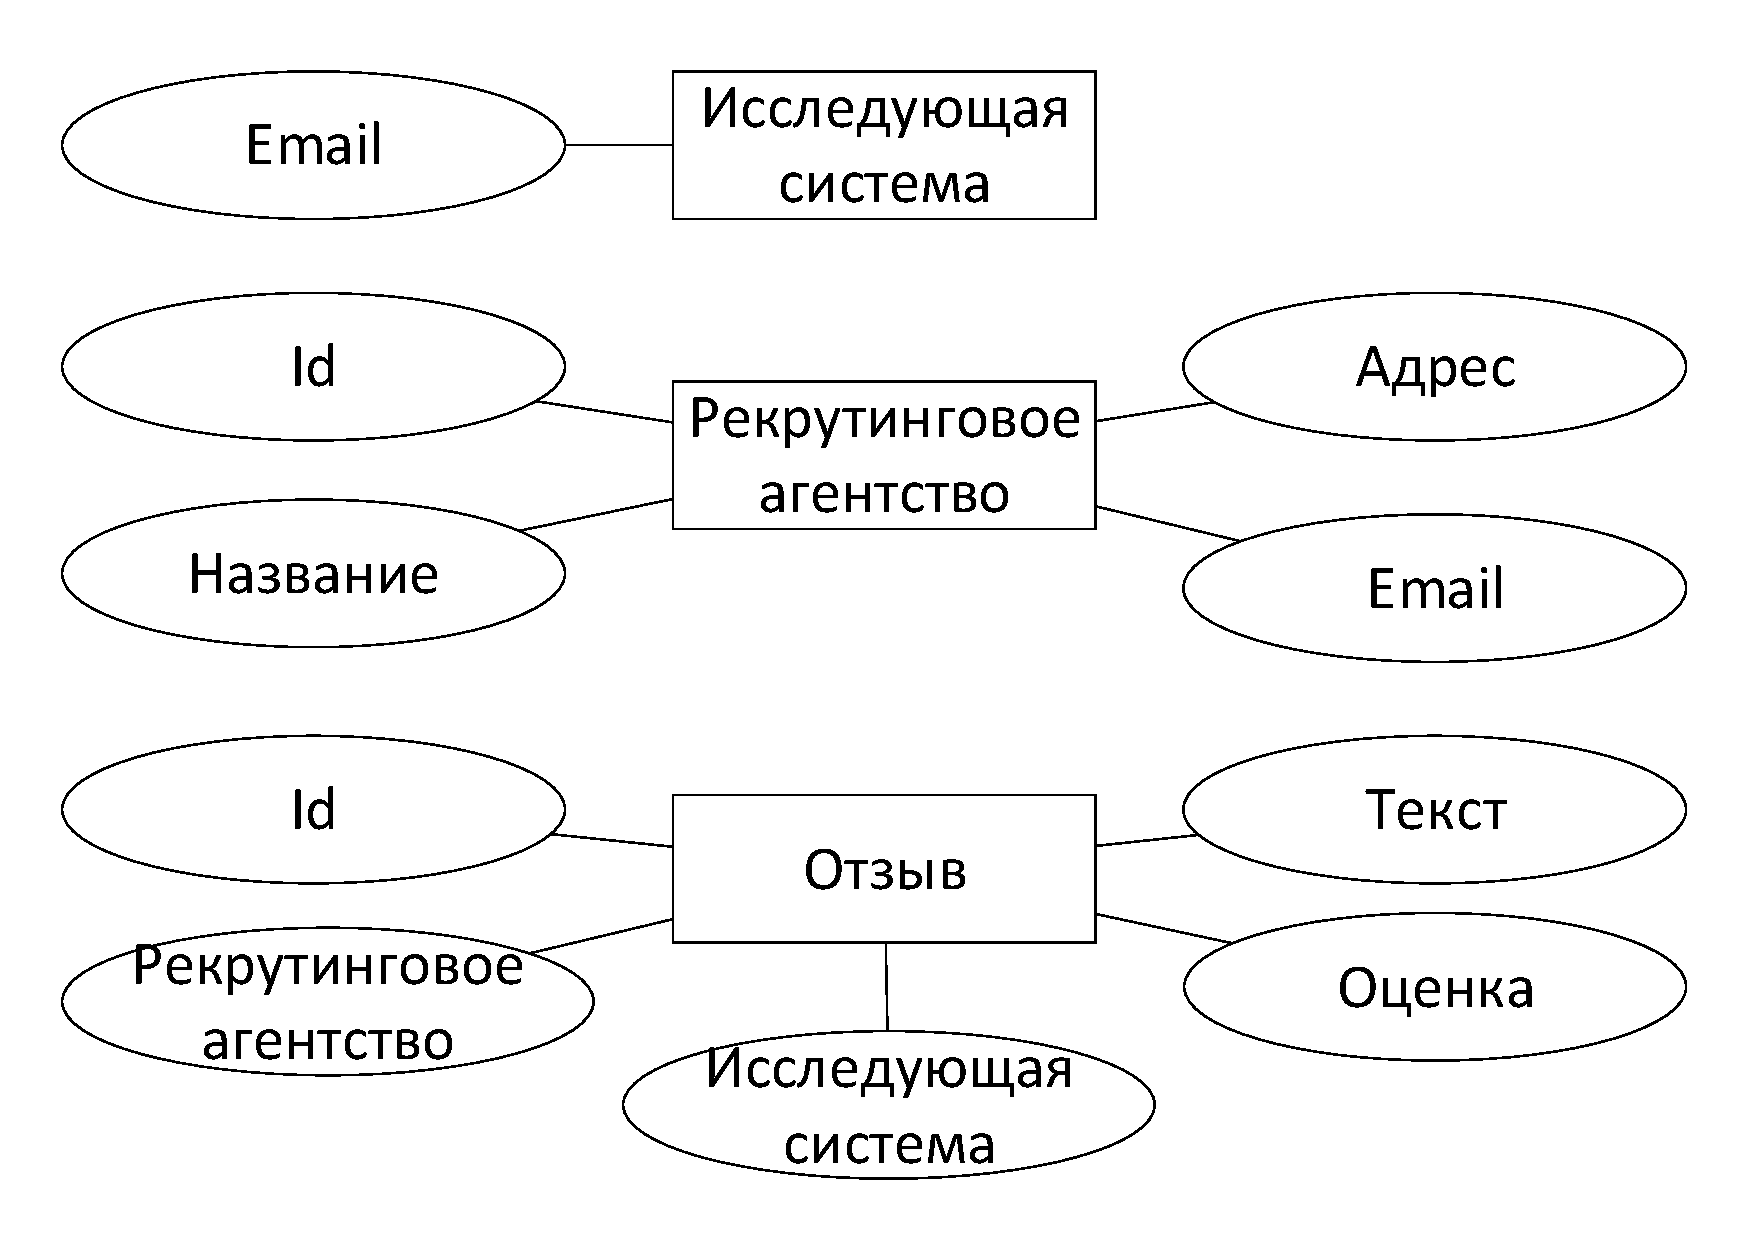
\includegraphics[width=\textwidth]{include/er-supervising-at.pdf}
\caption{Атрибуты сущностей контролирующей системы}
\label{fig:er-supervising-at}
\end{figure}

\begin{enumerate}
\item исследующая система — имеют email, оставляют отзывы;
\item рекрутинговое агентство — имеет название, адрес и email;
\item отзыв — имеет текст и оценку, оставляется исследующим агентством, относится к рекрутинговому агентству.
\end{enumerate}

\section{Система рекрутингового агентства}
Данные системы рекрутингового агентства содержат следующие сущности, связи которых представлены на рисунке ~\ref{fig:er-recruiting}, а описание атрибутов - на рисунке ~\ref{fig:er-recruiting-at}:

\begin{figure}[ht]
  \centering
  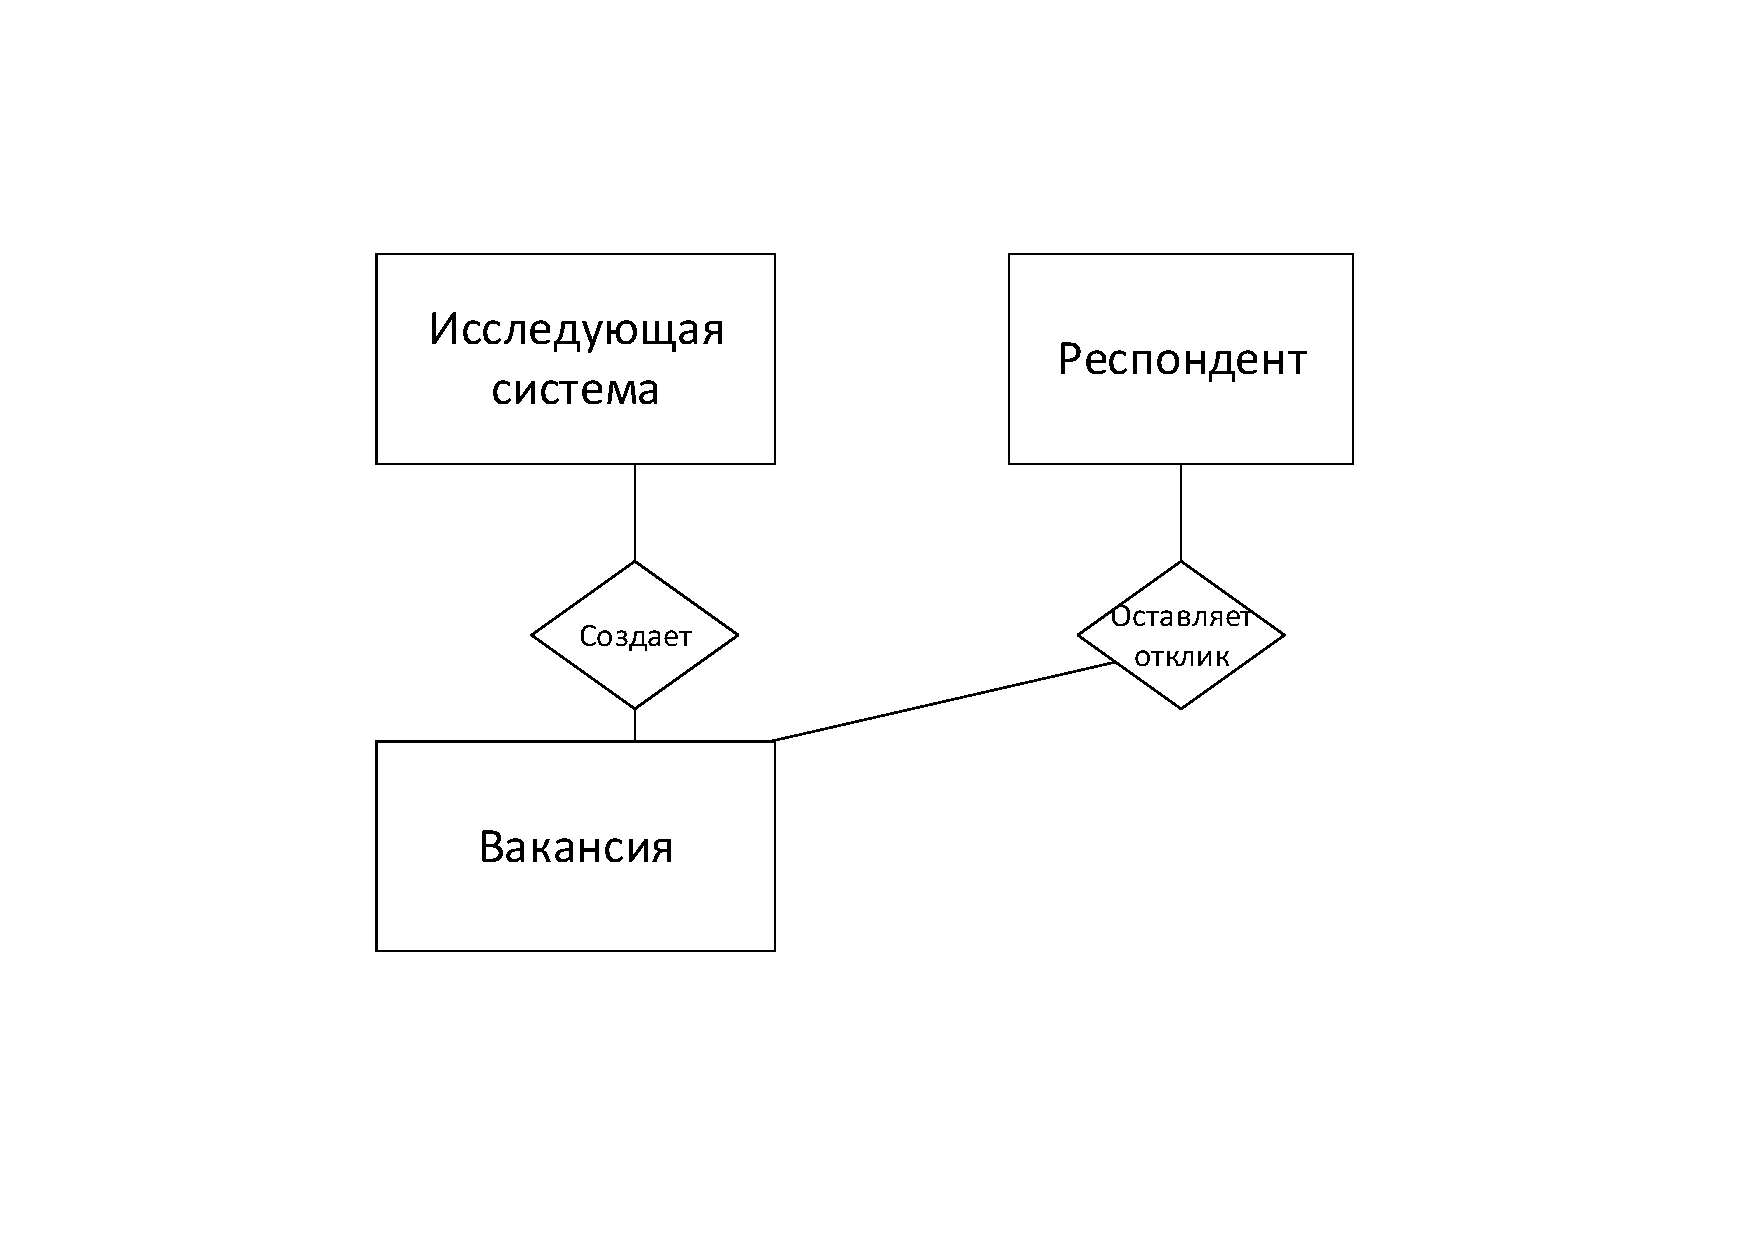
\includegraphics[width=\textwidth]{include/er-recruiting.pdf}
\caption{ER-диаграмма рекрутингового агентства}
\label{fig:er-recruiting}
\end{figure}

\begin{figure}[ht]
  \centering
  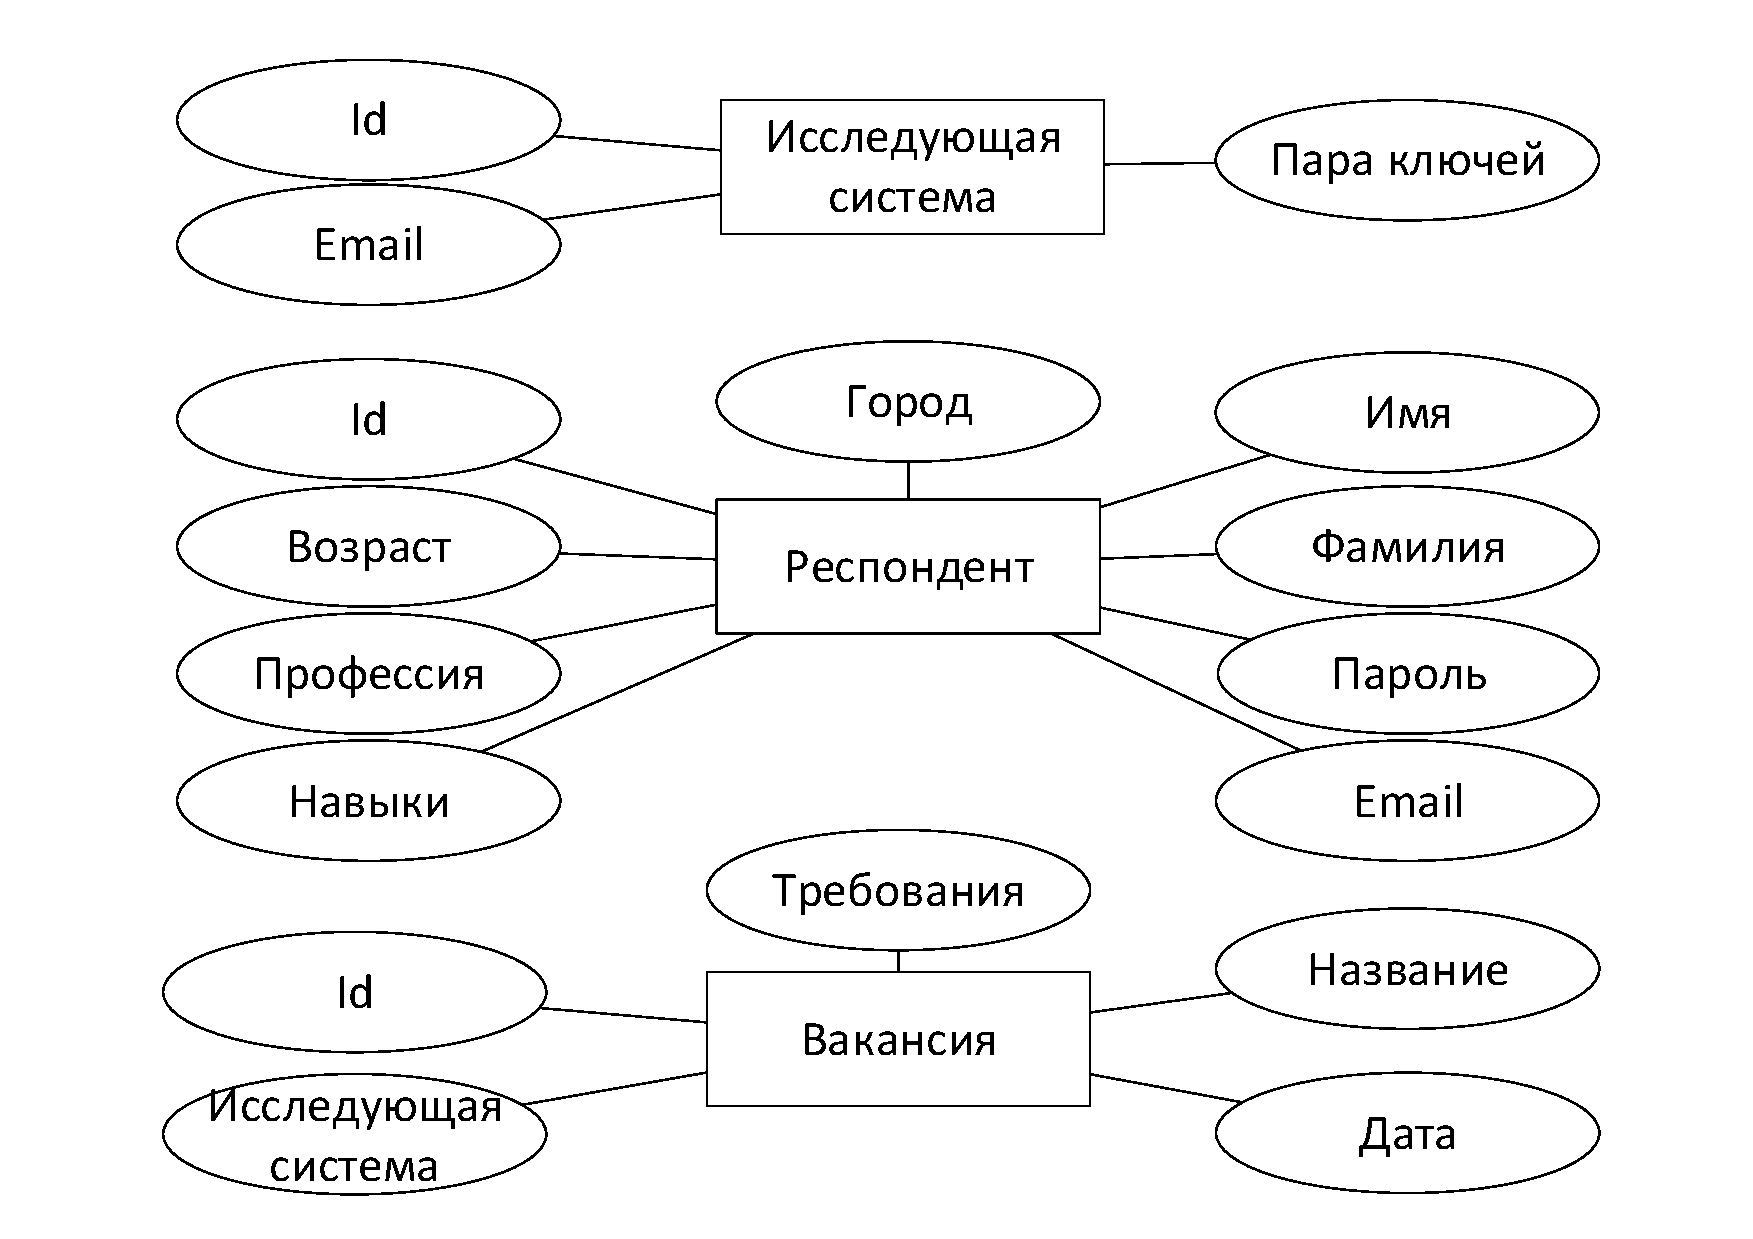
\includegraphics[width=\textwidth]{include/er-recruiting-at.pdf}
\caption{Атрибуты сущностей рекрутингового агентства}
\label{fig:er-recruiting-at}
\end{figure}

\begin{enumerate}
\item респондент — имеет такие атрибуты, как имя, фамилию, возраст, профессию, город, где он проживает, ключевые навыки, email и пароль к хэшированном виде; может оставлять отклики на вакансию;
\item вакансия — имеет название, дату, требования к респондентам;
\item исследующая организация — имеет email и пару ключей для подписи запросов; может создавать и закрывать вакансии;
\end{enumerate}

\section{Требования к шифрованию и цифровой подписи}
В рамках рассматриваемой работы сообщения должны передаваться по защищенным протоколам (HTTPS, SMTP+SSL). Сообщения в рекрутинговые агентства должны быть подписаны с помощью заранее заданного в конфигурации ключа.

%%% Local Variables:
%%% mode: latex
%%% TeX-master: "rpz"
%%% End:

\chapter{Технологический раздел}
\label{cha:impl}

В данном разделе описываются технические средства,  используемые при проектировании распределенной системы обработки информации. Также приведены результаты разработки и тестирования системы. 

\section{Среда разработки, язык программирования}
Разработка распределенной системы осуществлялась на языке Java с использованием MVC библиотеки Play!
Язык Java был выбран, потому что он является переносимым и имеет обширную библиотеку стандартных функций, значительно ускоряющих разработку приложений [2]. Фреймворк Play! был выбран, поскольку он содержит множество классов, помогающих в разработке Web-интерфейса участников и обмене сообщениями между ними [3]. Среда IntelliJ IDEA была выбрана, так как является кроссплатформенной средой разработки, поддерживает выбранный фреймворк и бесплатна для использования в учебных целях.

\section{Выбор протоколов взаимодействия}

\subsection{Протокол асинхронного взаимодествия}

В качестве протокола асинхронного взаимодействия был выбран протокол SMTP, так как он является одним из рекомендуемых кафедрой протоколов для выполнения курсового проектирования[4].

\subsection{Протокол синхронного взаимодействия}

В качестве протокола синхронного взаимодействия был использован протокол HTTP/REST, так как он является наиболее удобным протоколом для реализации в MVC-фреймворке и позволяет унифицированно взаимодейтсвовать как пользователю с системой, так и системам между собой.

\section{Выбор формата передачи данных}

В качестве формата запроса для синхронного протокола был использован формат x-www-form-urlencoded, поскольку его можно использовать как на стороне клиента (HTML-формы и Javascript), так и на стороне сервера.
В качестве формата ответа для синхронного протокола, а также запроса для асинхронного протокола был использован JSON, поскольку он является одним из широкоиспользуемых текстовых форматов и имеет развитые библиотеки как на стороне клиента, так и на стороне сервера.

\section{Диаграммы классов}

\subsection{Исследующая система}
На рисунке ~\ref{fig:class-survey} показаны классы для системы исследующей организации, за исключением моделей и автоматически сгенерированных представлений.
\begin{figure}[ht]
  \centering
  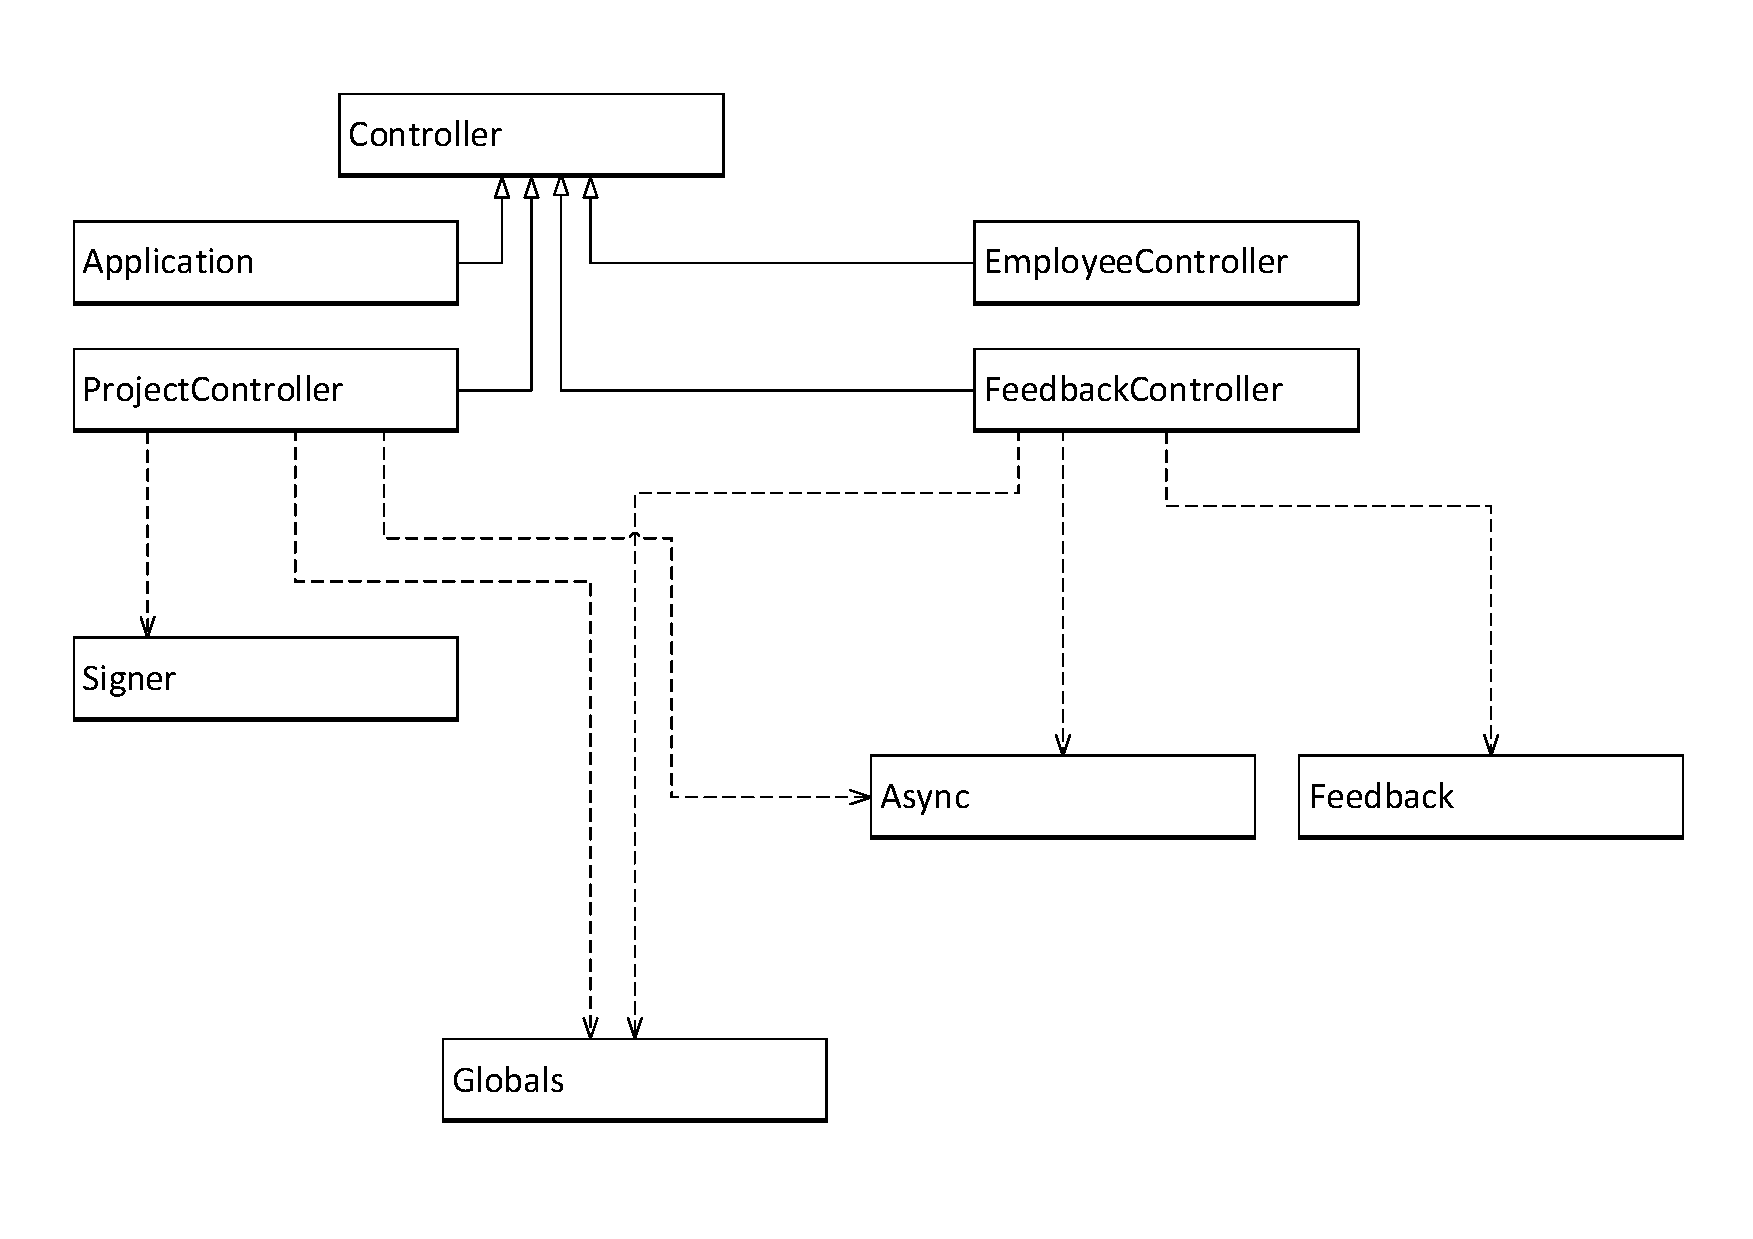
\includegraphics[width=\textwidth]{include/class-survey.pdf}
  \caption{Диаграмма классов исследующей системы}
  \label{fig:class-survey}
\end{figure}

\begin{enumerate}
\item Контроллеры:
\begin{enumerate}
\item Application - основной контроллер системы, реализующий функции авторизации через сервис Google.
\item EmployeeController - контроллер, осуществляющий добавление, редактирование и удаление респондентов.
\item ProjectController - контроллер, осуществляющий добавление и удалений проектов, создание и удалений вакансий в рекрутинговых агентствах и загрузку откликов.
\item FeedbackController - контроллер, осуществляющий кэширование данных о рекрутинговых агентствах, а также реализующий отправку отзыва об агентстве.
\end{enumerate}
\item Globals - модель, реализующая хранение системных переменных типа "ключ-значение". Используется для хранения времени последнего кэширования списка рекрутинговых агентств.
\item Async - класс, реализующий отправку асинхронных сообщений по протоколу SMTP.
\item Signer - класс, осуществляющий подпись синхронных и асинхронных запросов к рекрутинговым системам.
\item Feedback - класс, использующийся для промежуточного представления отзыва перед отправкой его контролирующей системе.
\end{enumerate}

\subsection{Контролирующая система}
На рисунке ~\ref{fig:class-supervising} показаны классы для системы контролирующей ассоциации, за исключением автоматически сгенерированных представлений.
\begin{figure}[ht]
  \centering
  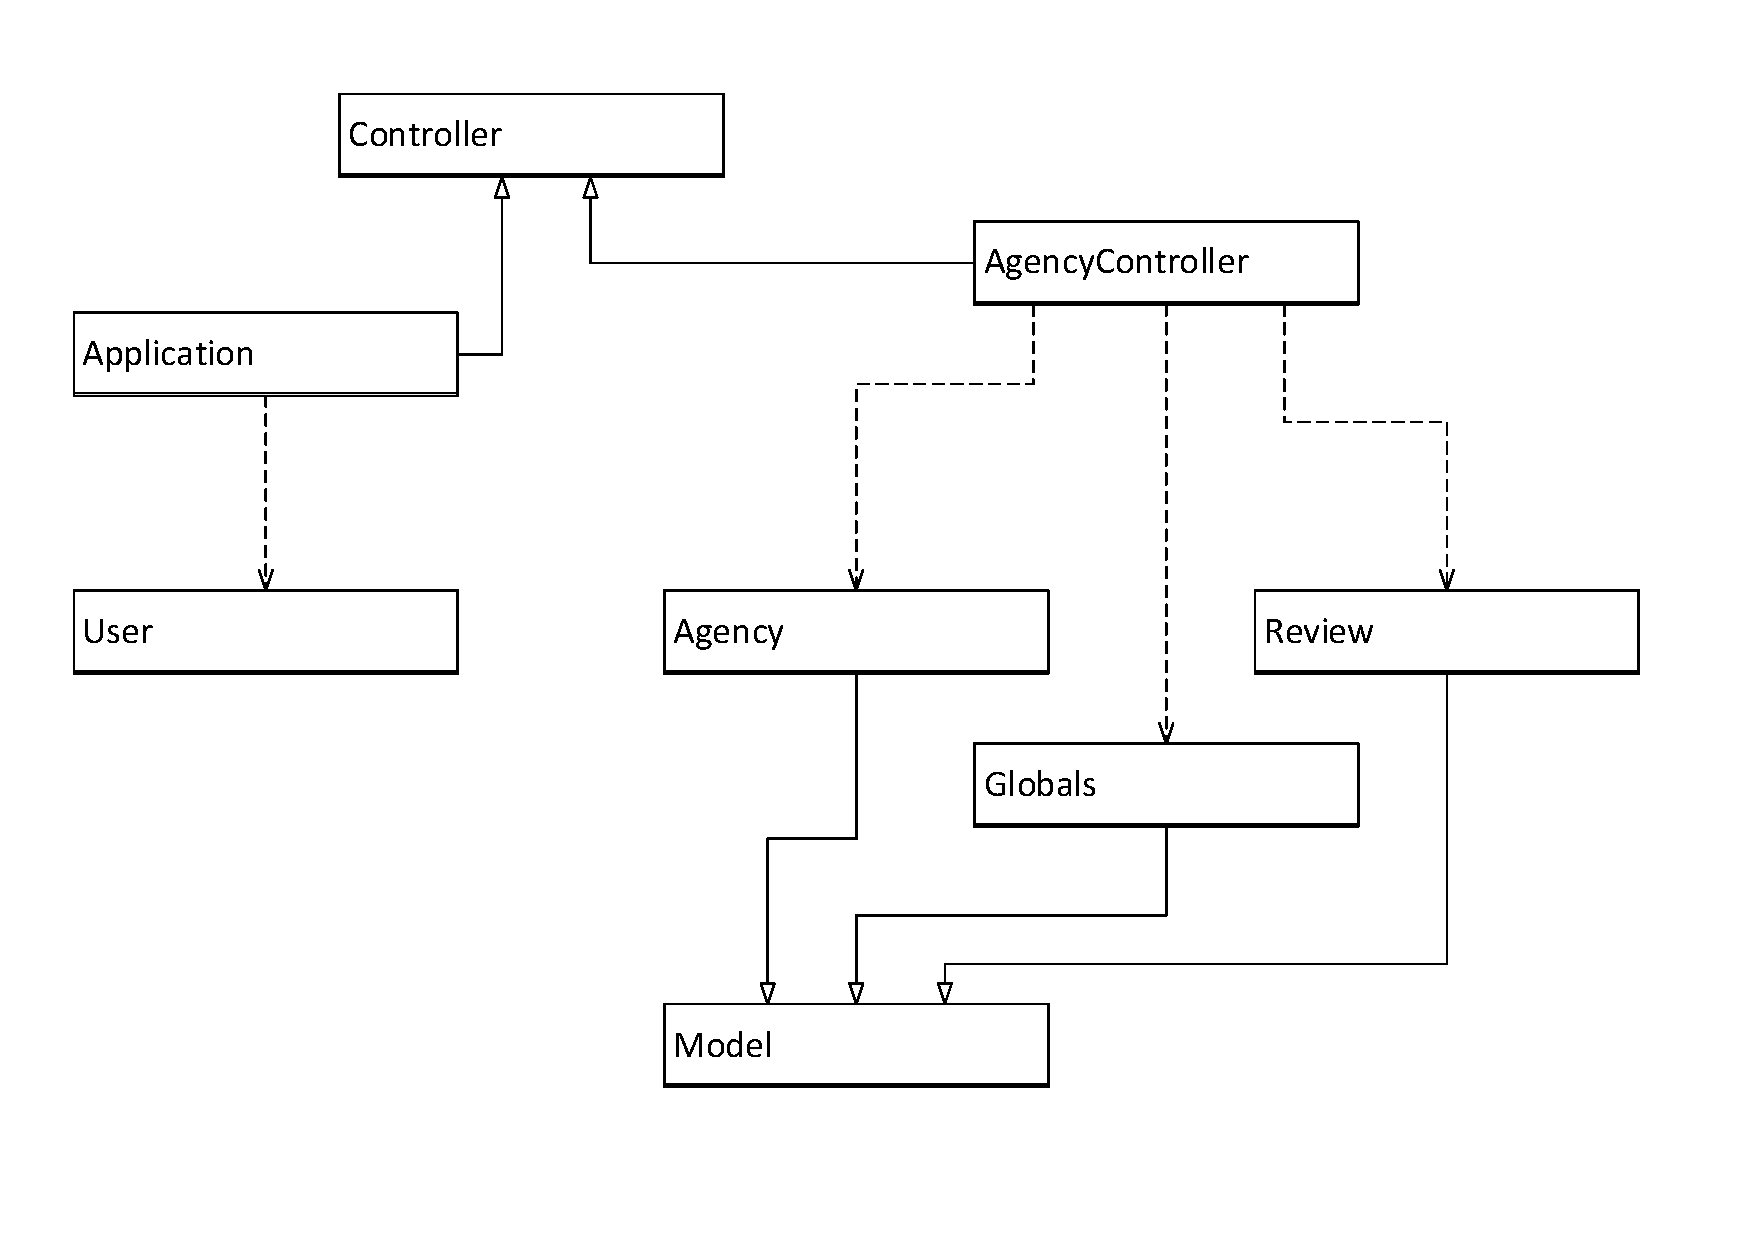
\includegraphics[width=\textwidth]{include/class-supervising.pdf}
  \caption{Диаграмма классов контролирующей системы}
  \label{fig:class-supervising}
\end{figure}

\begin{enumerate}
\item Контроллеры:
\begin{enumerate}
\item Application - основной контроллер системы, реализующий функции авторизации.
\item AgencyController - контроллер, реализующий добавление и удалений рекрутинговых агентств, а также получение отзывов о них.
\end{enumerate}
\item Модели:
\begin{enumerate}
\item Globals - модель, реализующая хранение системных переменных типа "ключ-значение". Используется для хранения последнего прочитанного сообщения POP3.
\item Review - модель, представляющая отзыв о рекрутинговом агентстве.
\item Agency - модель, представляющая рекрутингового агентство.
\end{enumerate}
\item User - класс, представляющий модель оператора контролирующей системы.
\end{enumerate}

\subsection{Рекрутинговая система}
На рисунке ~\ref{fig:class-recruiting} показаны классы для системы рекрутингового агентства, за исключением моделей и автоматически сгенерированных представлений.
\begin{figure}[ht]
  \centering
  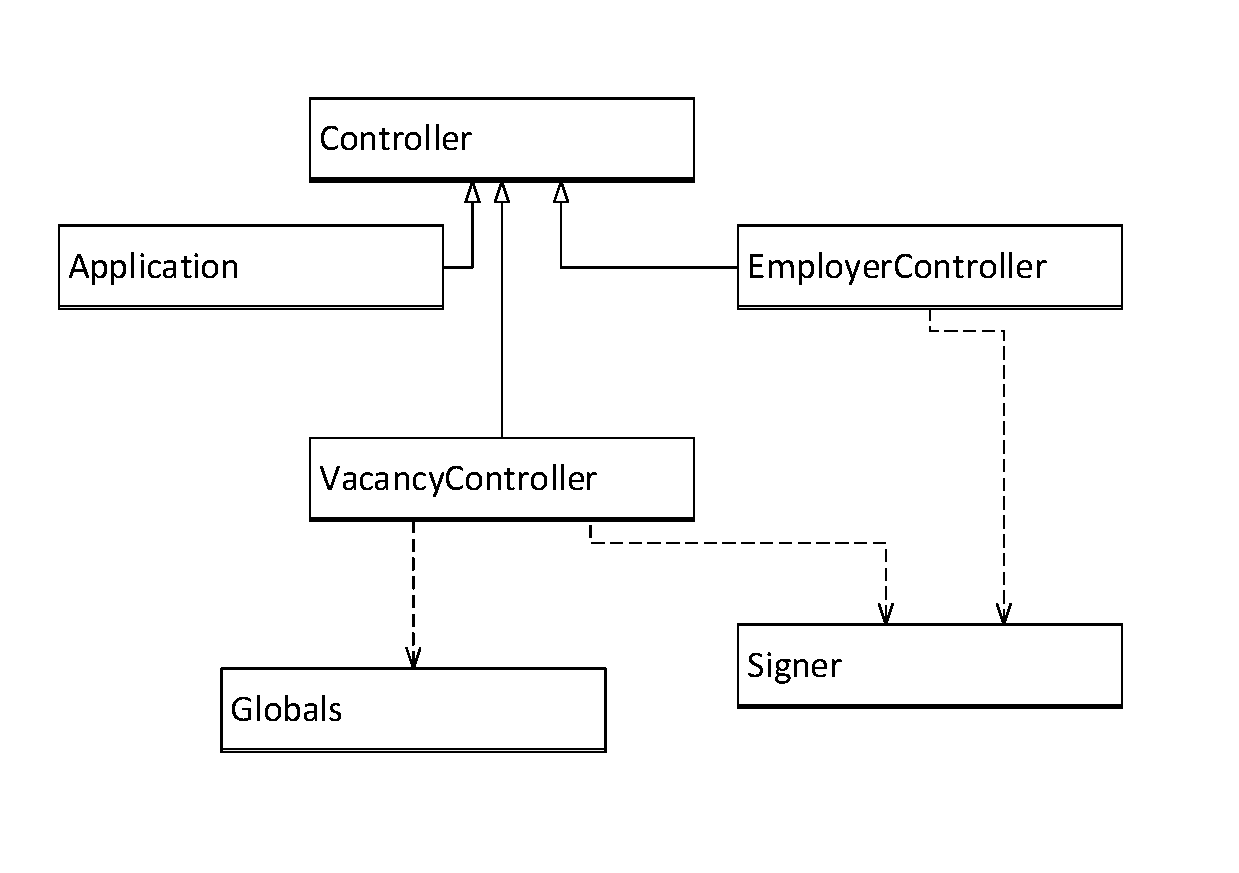
\includegraphics[width=\textwidth]{include/class-recruiting.pdf}
  \caption{Диаграмма классов рекрутинговой системы}
  \label{fig:class-recruiting}
\end{figure}

\begin{enumerate}
\item Контроллеры:
\begin{enumerate}
\item Application - основной контроллер системы, реализующий функции авторизации и регистрации.
\item EmployerController - контроллер, реализующий добавление и удалений работодателей и их секретных ключей.
\item VacancyController - контроллер, реализующий прием заявок на создание и удаление вакансий.
\end{enumerate}
\item Globals - модель, реализующая хранение системных переменных типа "ключ-значение". Используется для хранения последнего прочитанного сообщения POP3.
\item Signer - класс, осуществляющий проверку подписи синхронных и асинхронных запросов.
\end{enumerate}

\section{Реализация цифровой подписи}
В качестве алгоритма цифровой подписи использован алгоритм, аналогичный тому, что применяется в протоколе OAuth[1]. В качестве алгоритма шифрования для подписи использовался HMAC с хэш-функцией SHA256. Шаги составления подписи:
\begin{enumerate}
\item Для подписанных запросов добавляется параметр time, представляющий unix-time.
\item Формируется строка для подписи, представляющая из себя целевой URL, знак вопроса, затем параметры запроса в виде ключ=значение, отсортированные по алфавиту по ключу и разделенные знаком амперсанда. Для асинхронного запроса целевой URL и знак вопроса опускаются.
\item Формируется подпись - зашифрованная выбранным алгоритмом строка с использованием секретного ключа.
\item Далее подпись добавляется как параметр signature к остальным параметрам запроса.
\end{enumerate}

Для проверки подписи на принимающей стороне используется аналогичный алгоритм. Для выбора ключа запрос должен содержать email отправителя. Параметр signature не участвует в создании строки для подписи.

%%% Local Variables:
%%% mode: latex
%%% TeX-master: "rpz"
%%% End:


\backmatter %% Здесь заканчивается нумерованная часть документа и начинаются ссылки и

\Conclusion % заключение к отчёту

В результате проделанной работы мне удалось выяснить, что проделать работу как всегда надо больше.

%%% Local Variables: 
%%% mode: latex
%%% TeX-master: "rpz"
%%% End: 


% % Список литературы при помощи BibTeX
% Юзать так:
%
% pdflatex rpz
% bibtex rpz
% pdflatex rpz

\bibliographystyle{gost780u}
\bibliography{rpz}

\begin{thebibliography}{9}

% Даже для одного элемента ясно, что нужна приписка "Доступ получен"
\bibitem{JAVA}
	Java SE 6 Documentation, http://docs.oracle.com/javase/6/docs/

\end{thebibliography}


%%% Local Variables: 
%%% mode: latex
%%% TeX-master: "rpz"
%%% End: 


\appendix   % Тут идут приложения

\chapter{Тестирование системы}
\label{cha:appendix1}

\section{Тестирование Исследующей организации}

%TODO
Хорошо бы оттестировать хотя бы ее, потому что все запросы исходят отсюда, можно протестировать только здесь работу всеё системы, кроме асинхронных действий других.


%%% Local Variables: 
%%% mode: latex
%%% TeX-master: "rpz"
%%% End: 


\end{document}

%%% Local Variables:
%%% mode: latex
%%% TeX-master: t
%%% End:
